%%%%%%%%%%%%%%%%%%%%%%%%%%%%%%%%%%%%%%%%%%%%%%%%%%%%%%%%%%%%%%%%%%%%%%
% 基于 njuthesis 模板整理的本科毕业论文主文档
%%%%%%%%%%%%%%%%%%%%%%%%%%%%%%%%%%%%%%%%%%%%%%%%%%%%%%%%%%%%%%%%%%%%%%

\documentclass[
  type   = bachelor,
  degree = academic,
  fontset = fandol,
]{njuthesis}

\input{njuthesis-setup.def}

\usepackage{booktabs}
\usepackage{graphicx}
\usepackage{amsmath}
\usepackage{array}
\usepackage{multirow}
\usepackage{longtable}
\usepackage{tabularx}
\usepackage{float}

\newwrite\njuthesisauxguard
\AtBeginDocument{%
  \IfFileExists{\jobname.aux}{}{%
    \immediate\openout\njuthesisauxguard=\jobname.aux
    \immediate\closeout\njuthesisauxguard
  }%
}

\begin{document}
\maketitle
\raggedbottom

\begin{abstract}
随着 5G 网络中增强型移动宽带（eMBB）与超可靠低时延通信（URLLC）等异构业务的并发接入，如何在严苛的微时隙（Mini-slot）尺度下实现高效、稳定且满足服务等级协议（SLA）的切片资源分配，是无线接入网（RAN）系统设计的核心挑战。针对传统启发式打孔策略易导致局部资源过度剥削、而传统优化方法难以满足亚毫秒级实时调度的瓶颈，本文基于自建的 5G NR 离散化时序仿真环境，提出了一种面向风险规避的深度强化学习资源分配模型。

本文将 URLLC 的动态抢占过程建模为容忍度感知的马尔可夫决策过程（MDP）。针对单目标优化可能带来的局部资源过度使用问题，本文提出一种基于近端策略优化（PPO）的频域负载均衡调度算法（VarPPO）。该算法在状态空间中融入队列动态与 eMBB 码字理想可靠性裕度，并在奖励函数中引入打孔计数与剩余裕度的多维方差惩罚项。通过在可用频段内分摊打孔压力，引导智能体学习兼顾时延约束与传输稳定性的调度策略。

在当前单小区、完美 CSI 辅助观测的仿真场景下，实验结果表明，相较于静态打孔、启发式轮询以及基线 PPO 算法，VarPPO 在 URLLC 时延违约率基本持平的前提下，对 eMBB 链路中断率、剩余裕度方差等指标有一定改善。其中，相较于基线 PPO 的提升幅度较为温和，主要体现为 eMBB 侧风险分布更加平滑。本文所构建的仿真框架与算法实现，可为后续混合业务切片调度研究和面向 O-RAN 控制器的策略验证提供仿真参考。

\end{abstract}

\begin{abstract*}
With the concurrent provisioning of heterogeneous services, such as Enhanced Mobile Broadband (eMBB) and Ultra-Reliable Low-Latency Communication (URLLC) in 5G networks, achieving efficient, stable, and Service Level Agreement (SLA)-compliant slice resource allocation at the stringent mini-slot scale remains a fundamental challenge in Radio Access Network (RAN) design. Traditional heuristic puncturing strategies are prone to over-exploiting local resources, while conventional mathematical optimization methods fail to meet the stringent sub-millisecond real-time scheduling constraints. To address these bottlenecks, this paper proposes a risk-averse deep reinforcement learning (DRL) resource allocation framework based on a customized 5G NR discretized time-series simulation environment.

The dynamic preemption process of URLLC is formulated as a tolerance-aware Markov Decision Process (MDP). To mitigate local overuse of frequency resources under single-objective optimization, we propose a frequency-domain load-balancing scheduling algorithm, termed VarPPO, built upon Proximal Policy Optimization (PPO). VarPPO incorporates URLLC queue dynamics and the ideal reliability margins of eMBB codewords into its state space. It further integrates a multi-dimensional variance penalty into the reward function to account for puncturing counts and remaining reliability margins. By distributing puncturing pressure across available frequency bands, the agent is guided to learn a scheduling policy that balances latency constraints and transmission stability.

Under the current single-cell simulation setting with perfect-CSI-assisted observations, the results show that VarPPO improves eMBB outage rate and remaining-margin variance while keeping the URLLC violation rate broadly comparable to the baseline PPO. The improvement over PPO is moderate and is mainly reflected in smoother eMBB-side risk distribution. The simulation framework and implementation in this study provide a reproducible reference for subsequent research on mixed-traffic slice scheduling and for future policy validation toward O-RAN controllers.

\end{abstract*}

\tableofcontents
\mainmatter

% !TeX root = ./main.tex
\chapter{绪论}\label{ux7b2cux4e00ux7ae0-ux7eeaux8bba}

\section{研究背景及意义}\label{11-ux7814ux7a76ux80ccux666fux53caux610fux4e49}

\begin{figure}[H]
\centering
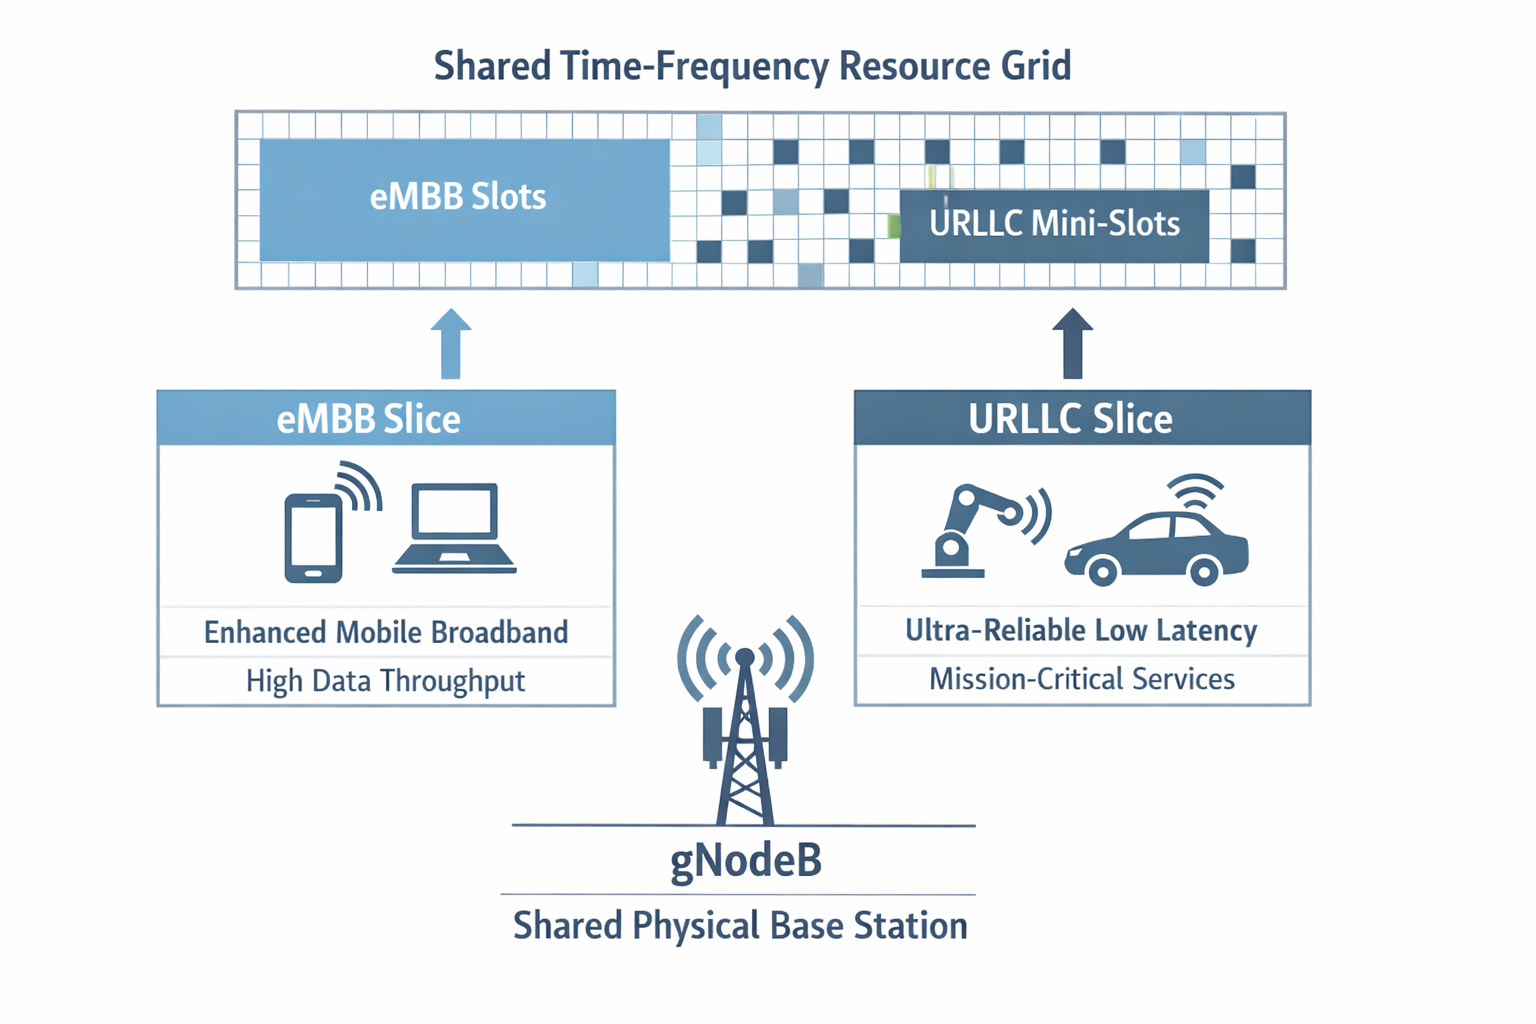
\includegraphics[width=0.9\textwidth]{解释5G网络切片的基本概念.png}
\caption{5G 网络切片的基本概念}
\label{fig:5g_network_slicing_concept}
\end{figure}





随着5G移动通信网络在全球铺开，B5G 和 6G 的研究也开始被提出，无线通信系统面对的业务类型，比过去复杂得多，要求也“极端”\cite{luong2019, dai2025}得多。国际电信联盟通常把 5G 的典型应用场景分成eMBB、URLLC和mMTC三类 \cite{popovski2018, hua2020}。这三类场景关注的重点可不一样，有时候甚至会互相“打架”。eMBB 主要服务于超高清视频、虚拟现实这类数据量很大的应用，它更关心系统吞吐量和频谱效率，希望网络能尽可能“多传、快传”。URLLC 则面向工业自动化、自动驾驶、远程医疗等关键任务，它更看重低时延和高可靠性，端到端时延需要低到 1 毫秒（ms）左右，传输可靠性还要达到 $10^{-5}$ 量级。URLLC 大都工作在短包传输情形，码长非常有限，所以可靠性、时延和资源占用之前的联系也就更强；天线、带宽、功率等资源如何合理地分配，也就非常关键\cite{sun2019short}。相较而言，mMTC 的服务对象是海量的低功耗的物联网设备，它更关注大规模终端的同时接入\cite{huang2022deluxe, filali2022}。所以，在同一套有限的物理网络基础设施上，同时照顾这些差异很大的业务需求，已经成为 5G 以及未来 6G 系统设计中绕不开的问题\cite{popovski2018, feng2020}！

为了解决这类矛盾，一些科学家提出了网络切片（Network Slicing）这个技术，这个技术也逐渐成长成下一代无线网络资源管理中的重要思路\cite{hua2020, filali2022}。那么，网络切片是什么呢？简单的说，它指的是是在同一套物理网络上，划出多个逻辑上相互隔离、服务目标不同的虚拟网络，也就是“切片”\cite{filali2022, dai2025}，每个切片可以根据自己的业务特点，配置不同的资源，并满足对应的服务等级协议（Service Level Agreement）要求\cite{hua2020, alcaraz2023}。

放到无线接入网（Radio Access Network）中来看，切片资源管理一般可以分成两个层次。第一层是比较宏观的资源划分，比如在不同业务切片之间分配带宽、功率等资源，让它们既能共享网络，又不会互相干扰太严重；第二层则更细一些，主要是在某个切片内部，给具体用户安排时频资源块（Resource Block）\cite{filali2022, dai2025}。不过，在真实的 5G RAN 部署中，切片资源分配从来就不是一个静态的问题，这是因为业务流量会不断变化，多个 QoS指标之间也就会互相牵制，再加上各种系统约束，问题本身就具有很强的动态性和耦合性\cite{choi2024, alcaraz2023}。尤其是在 URLLC 和 eMBB 混合存在的情况中，这种矛盾只会更加明显\cite{alsenwi2021, saggese2021}。

URLLC 流量有一个很典型、很有意思的特点：它不一定一直来，但一旦来了，就必须马上处理。如果单独给 URLLC 预留一块固定频段，虽然可以保证它有资源可用，但在 URLLC 没有数据到达的时候，这部分频谱就会空着，造成比较明显的浪费\cite{alsenwi2021, sohaib2023}。为了解决这个问题，3GPP 标准中引入了动态抢占（Preemption）机制。这个机制可以实现 URLLC 数据突然到达时，基站临时打断正在传输的 eMBB 资源，把这部分资源先让给 URLLC 使用\cite{anand2020, huang2022deluxe}。从比较底层的角度看，这种抢占的物理后果是对 eMBB 码字的局部打孔（Puncturing）。换句话说，抢占描述的是基站侧“把资源让出来”的调度动作，而打孔描述的是这个动作在 eMBB 物理层上造成的局部擦除效果。
这样做我感觉确实可以更好地保证 URLLC 的实时需求，但是 eMBB 的传输完整性也肯定会被破坏，被打孔的位置多了以后，eMBB的吞吐量会出现波动，严重的话
甚至有可能会导致底层业务中断\cite{alsenwi2021, saggese2021}。

面对这样的复杂资源的竞争环境，传统的资源分配的算法会遇到不小的压力。传统算法根据我的总结分为两类：一类常见方法是启发式算法，比如比例公平调度，这类方法实现起来比较简单，也有一定的工程基础，但它们在面对毫秒级流量变化和多维度的服务质量约束
时，反应不够灵活，也很难提前判断后续风险\cite{dai2025}；另一类方法则是数学优化，比如混合整数非线性规划（MINLP）或连续凸近似（SCA），
这些方法通常来自比较严谨的数学的推导，理论上的确是可以得到较好的解，可惜其实这类问题在实际中常常属于 NP-hard 类型，求解的复杂程度特别高。
对于 RAN 中毫秒级的在线调度来说，这样的计算开销很难接受\cite{feng2020, sohaib2023}。

近年来，深度强化学习（Deep Reinforcement Learning）的发展，为动态切片资源管理提供了一种新的、可能的方向\cite{luong2019, hua2020}。DRL 可以把
资源分配过程看成一个马尔可夫过程的问题，智能体通过不断和网络环境交互，根据状态选择动作，再从反馈中慢慢学出一套近似调度策略\cite{filali2022, choi2024}。这
样一来，模型就可以完全不用依赖精确的数学表达式，也不需要每次在线调度时都重新求一个十分复杂的优化问题了。DRL 的另一个优势在于，它可以先离线训练，再在线推理
。也就是说，比较耗时的学习过程可以提前完成，真正部署时只需要让训练好的模型快速给出接下来要做的步骤。如果再配合边缘计算节点的硬件加速能力，DRL 非常希望
减轻传统优化方法在线求解开销大的问题，并用于毫秒级实时调度场景的探索\cite{filali2022, alcaraz2023}。已有研究的实测结果显示，在神经网络规模合理的情况下，训练后的 PPO智能体完成一次资源调度的平均推理时间大约可以控制在 0.3 到 3.0 毫秒之间，具体数值取决于底层硬件算力\cite{saggese2021}。甚至如果进一步使用经过高度优化的 CPU/GPU 混合架构，基于深度学习的物理层调度有可能能够做到满足 5G NR 中低于 100μs 的严苛的实时性的要求\cite{huang2022deluxe}。从这些研究可以看出，DRL 的在线推理能力，为处理 URLLC 对时延非常敏感的调度问题提供了一个可以参考的方向\cite{huang2022deluxe, saggese2021}。本文关注的问题也正是基于这一点：在尽量保证 URLLC服务质量的前提下，如何利用 DRL 算法压低“动态抢占”和物理层打孔对 eMBB 业务带来的冲击，让 eMBB 的吞吐量不只维持在较高水平，还能尽量保持稳定。

与此同时，开放无线接入网（O-RAN）架构的推广，也给 RAN 智能调度提供了更清晰的工程入口\cite{dai2025}。O-RAN 通过引入近实时无线接入网智能控制器，并开放 E2 、E4等等标准化接口，能够使得深度强化学习这类智能调度器可以以 xApp 微服务的形式接入无线接入网控制流程\cite{dai2025, choi2024}，这样就有点像是把原本一体化的黑盒子拆开、分层了。在这个背景下，本文选择在单小区下行环境中建立可复现的仿真框架，并设计、对比基于 DRL 的调度策略，这样的工作可以为后续面向 O-RAN 的 6G 智能调度系统设计、SLA 鲁棒性验证以及工程化评估提供一定的仿真参考，甚至在未来很有机会能够应用在真正的基站中。



\section{国内外研究现状}\label{12-ux56fdux5185ux5916ux7814ux7a76ux73b0ux72b6}

\subsection{传统无线资源管理与网络切片调度}\label{121-ux4f20ux7edfux65e0ux7ebfux8d44ux6e90ux7ba1ux7406ux4e0eux7f51ux7edcux5207ux7247ux8c03ux5ea6}

无线资源的管理的最传统的方式，就是使用启发式调度器和数学规划模型。这些调度器和模型中，比例公平（Proportional Fair, PF）算法最具有代表性，这个算法的原理就是对信道质量与历史吞吐量加权折中，而这个算法也在 LTE 及早期 NR 系统中广泛的部署了\cite{kavehmadavani2024}。然而，这类调度器虽然看起来非常的简单，但是从本质上来说，这种算法是为单一业务类型或相对稳定的网络负载设计的，当网络迈向5G时代后，面对 URLLC与 eMBB的毫秒级的突发性的资源竞争，这种旧方法的处理能力明显不足了\cite{feng2020}。

最开始探索URLLC和eMBB的联合调度问题的思路，是通过静态或半静态的正交频谱分配将两类流量物理隔离。很明显，这种思路基本承袭的就是无线资源管理的传统方法。然而，URLLC包本身具有高度偶发性，这会使得在无 URLLC 业务时，可能会有超过百分之60的频谱资源被白白搁置\cite{ji2018, popovski2018}！另一种思路从网络切片供给角度来建模这个新问题，将覆盖范围、云网络资源与无线约束统一在线性规划的框架中来分析\cite{luu2020}。此外，也有一些比较小众的研究采用李雅普诺夫优化、连续凸近似（SCA）或半定松弛（SDR）等联合优化手段，在理论层面取得了显著的性能上限的提升；然而这些方法的实时求解开销往往过大，很大程度上只能永远停留在理论上，在真实基站调度场景中根本无法直接落地\cite{feng2020, yang2021bursty}。

\subsection{深度强化学习在资源管理中的应用}\label{122-ux6df7ux5408ux5f3aux5316ux5b66ux4e60ux5728ux8d44ux6e90ux7ba1ux7406ux4e2dux7684ux5e94ux7528}

为了补上传统优化方法在实时性上的不足，深度强化学习慢慢进入无线通信领域，并被用到功率控制、频谱共享、路由选择、动态调度等多类问题中，这类方法能根据网络状态变化调整决策方式，因此表现出了较好的自适应能力\cite{luong2019}；较早一批DRL研究通常采用基于价值的方法（如 Deep Q-Network, DQN），把资源块分配处理成离散决策，从而提升系统整体吞吐量\cite{luong2019, li2020}；后来，研究者又逐渐把策略梯度类方法（如 DDPG、A2C、PPO）引入进来，用来处理连续发射功率调节等更细的动作空间\cite{luong2019, hua2020}。在多切片场景中，也有研究设计了双层DRL框架，上层智能体负责切片之间的整体资源划分，下层智能体负责切片内部面向用户的具体调度\cite{setayesh2022, filali2022}。

在变化很快的车联网场景中，DRL也常被用来处理URLLC链路可靠性约束，以及车辆高速移动带来的资源起伏问题，面向IoV的强化学习方案可以在满足URLLC通信约束的同时，提高车辆链路容量\cite{yang2019iov}；引入D2D通信的虚拟化车载网络资源切片方案，则把DRL的决策范围进一步扩大到车载网络的资源管理中\cite{sun2020vehicular}。除车联网外，DRL还被用到意图感知网络中的服务质量调度\cite{nahum2024}，以及链路级的细粒度切片执行\cite{wang2022linkslice}等方向；改进型DQN通过“优先经验回放”和"奖励整形"，能够支撑预测性切片与自适应资源分配\cite{yagcioglu2026}，多智能体深度强化学习也能在只掌握延迟信道状态信息的情况下，实现接近“集中式优化水平”的分布式功率控制\cite{nasir2019}。

然而，上述早期 DRL 工作的奖励函数设计大多以最大化系统平均吞吐量为目标。在URLLC-eMBB混合场景中，这种设计容易产生"赢者通吃"现象，即系统为维护整体指标而过度牺牲信道条件较差的边缘eMBB 用户\cite{alsenwi2021}。

\subsection{混合切片场景中的风险规避与打孔研究}\label{123-ux6df7ux5408ux5207ux7247ux573aux666fux4e2dux7684ux98ceux9669ux89c4ux907fux4e0eux52a8ux6001ux6253ux5b54ux7814ux7a76}

这5年以来，混合切片场景下的研究重心也逐渐从单纯提升平均吞吐量转向兼顾可靠性、稳定性与服务连续性\cite{bennis2018}。在这一方向上，我认为Alsenwi 等人的工作具有很强的代表性\cite{alsenwi2024distributed}，他们将金融领域的条件风险价值（CVaR）的这个概念引入无线资源分配的过程中来，把 eMBB 速率的方差项作为惩罚项，作为整个系统优化的一部分\cite{alsenwi2019risk}。这种风险规避调度策略在保证 URLLC 绝对优先级的同时，有效避免了信道较差的 eMBB 用户遭受极端打孔的过度剥削，也验证了将风险度量嵌入 DRL 奖励函数对提升系统稳定性的实际价值。另一方面，我感觉Saggese 等人提出了一种基于 PPO 的 URLLC 数据管理方案\cite{saggese2021}也非常的有价值。这个方案的核心思路是：训练 PPO 智能体，让智能体来决策URLLC包打孔eMBB包的哪些位置，最终能够让传输损耗最小化。在奖励函数中加入 eMBB 码字中断惩罚项后，该方案在严格满足 URLLC 时延约束的前提下，有效降低了 eMBB 业务的中断率。

\subsection{O-RAN 架构下的智能化调度部署}\label{124-o-ran-ux67b6ux6784ux4e0bux7684ux667aux80fdux5316ux8c03ux5ea6ux90e8ux7f72}

伴随 O-RAN 架构慢慢在成熟，智能调度算法的工程落地路径也变得更加的清晰\cite{bonati2021}。O-RAN 的开放接口（E2、O1、A1）与分层控制环路机制，可以让DRL调度器以 xApp（部署于 Near-RT RIC 的微服务级应用）或 rApp（部署于 Non-RT RIC）的形式原生的嵌入无线接入网络，这是一个前所未有的伟大创举\cite{dai2025}。在切片资源的管理层面，已有研究将 PRB与功率分配纳入开放接口下的切片优化，以满足 eMBB、URLLC 与 mMTC 的差异化需求\cite{motalleb2023}。受约束的多个智能体的强化学习也有被用于适应可变切片数量以及降低服务质量违约的风险\cite{zangooei2024}；联邦深度强化学习技术则通过分布式的本地决策，减少了集中式控制的通信开销，为将来的6G RAN 切片编排提供了更好的可扩展性\cite{rezazadeh2023}。此外，也有研究通过DRL算法持续监控 RAN 性能指标、将运营商（例如中国电信、中国移动）的服务质量保证作为硬性约束嵌入训练反馈，实现了兼顾鲁棒性与隔离性的切片资源分配\cite{alcaraz2023}。

综合以上文献来看，DRL 辅助切片管理和 O-RAN 概念验证方面的工作到目前为止已经相当的丰富，我最后能找到的研究问题是：在单小区下行混合打孔场景下，建立一个细粒度、可复现、且与 5G 标准（时隙与微时隙嵌套结构）高度契合的仿真框架，并对不同 DRL 策略（尤其是 PPO）的稳定性与吞吐量表现进行系统比较。下表从状态空间、动作空间、奖励函数设计及关键特性等等维度对本文引用的核心文献进行对比，并清晰的标注了本文工作的定位，以说明本文在现有研究格局中的创新切入点。下表中，有一个概念值得我单独说明，既“广义优势估计（Generalized Advantage Estimation, GAE-$\lambda$）”，这是一种用于降低策略梯度方差的优势函数估计方法，通常与 PPO 配合使用。
\begin{table}[htbp]
\centering
\small
\setlength{\tabcolsep}{4pt}
\caption{基于强化学习的混合切片资源分配代表性文献对比}
\label{tab:literature_comparison}
\renewcommand{\arraystretch}{1.3}
\begin{tabularx}{\textwidth}{@{}>{\raggedright\arraybackslash}p{0.14\textwidth}>{\raggedright\arraybackslash}p{0.18\textwidth}>{\raggedright\arraybackslash}X>{\raggedright\arraybackslash}p{0.12\textwidth}>{\raggedright\arraybackslash}X@{}}
\toprule
\textbf{文献} & \textbf{动作空间定义} & \textbf{奖励设计与方差控制} & \textbf{算法} & \textbf{局限性} \\
\midrule
\cite{anand2020} & 离散打孔（是/否） & 违约率与吞吐量 \newline (未考虑方差) & 数学优化 & 依赖完美CSI，难适应在线动态 \\
\cite{saggese2021} & 离散频段打孔位置 & 中断与时延惩罚 \newline (无方差惩罚，易致单点崩溃) & PPO + GAE & 未评估跨负载泛化；易致局部链路过度剥削（Over-exploitation） \\
\cite{alsenwi2024distributed} & 混合分配与打孔 & 速率均值与方差权衡 \newline (显式约束方差) & 多智能体 AC & 架构实现复杂度极高；缺 OOD 测试 \\
\cite{cai2024} & 连续功率/RB 分配 & 功率与 RU 约束 \newline (未关注稳定性) & 预测加权 DRL & 预测模块误差易累积，影响性能 \\
\cite{dai2025} & 宏观切片资源建议 & SLA 违反率惩罚 \newline (未关注稳定性) & 深度回声 DQN & 偏宏观部署，缺乏底层打孔物理建模 \\
\textbf{本文工作定位（提出方法）} & \textbf{离散频段打孔位置} & \textbf{综合时延与中断惩罚 + 频域打孔负载均衡} & \textbf{PPO + \newline GAE-$\lambda$} & \textbf{限于单小区场景；状态维度随用户上升} \\
\bottomrule
\end{tabularx}
\end{table}

从表~\ref{tab:literature_comparison} 的对比分析可以看出，现有基于 DRL 的调度方案多聚焦于吞吐量最大化或单一的违约率控制，对频域打孔压力分布与高负载迁移下系统表现的讨论仍有拓展空间。如何在保障高优先级业务时延约束的同时，缓解打孔负载在少数频域资源上的集中，是本文重点研究的问题。



\section{主要研究内容}\label{13-ux4e3bux8981ux7814ux7a76ux5185ux5bb9ux4e0eux8bbaux6587ux7ed3ux6784}

\begin{figure}[H]
\centering
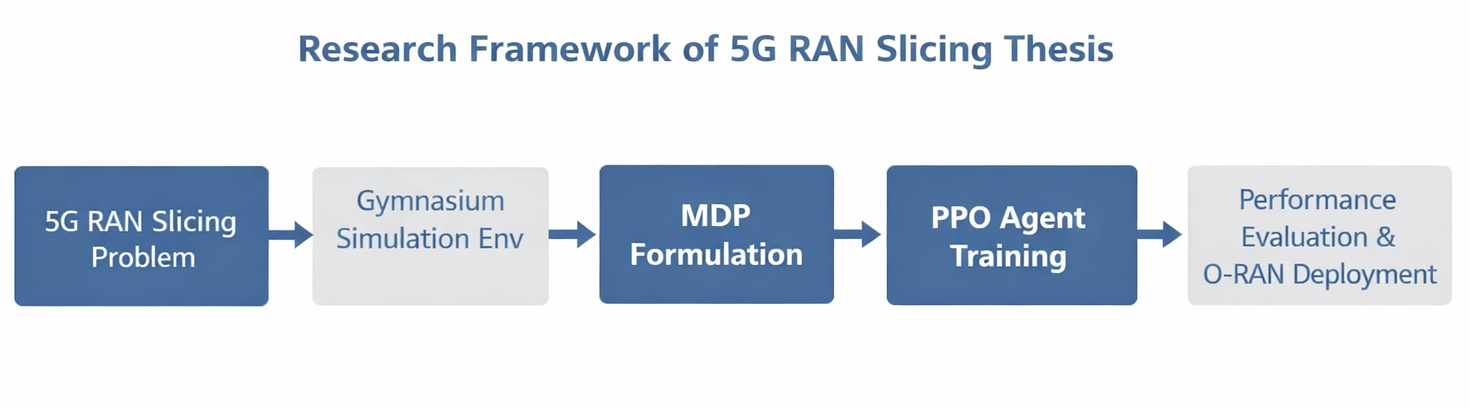
\includegraphics[width=0.9\textwidth]{研究内容与整体框架.png}
\caption{研究内容与整体框架}
\label{fig:research_framework}
\end{figure}

5G无线接入网中URLLC和eMBB业务的混合调度很容易会引发激烈的资源冲突。为了在保障绝对优先级的打孔机制下，尽可能维持系统整体的通信稳定性，我在这篇文中重点研究了如何利用深度强化学习（DRL）来优化RAN切片的资源分配。具体的研究工作如下：

第一步是构建仿真环境基座。我基于openai最新的Gymnasium框架，开发了一个单小区下行链路的强化学习仿真环境。整个环境可以很真实的还原5G标准里的Slot和Mini-slot两级时间尺度，并将信道衰落、动态打孔造成的码字中断等底层物理机制纳入到观测闭环中。

第二步是复杂的马尔可夫过程的建模与容忍度感知。我考虑到真实信道环境存在容忍度差异（这是因为有的人的手机在信号好的地方，有的人在信号不好的地方），把动态调度转化成了一个状态丰富的马尔可夫决策过程。在完美CSI假设的辅助下，我的建模能够让系统实时捕获URLLC队列积压、剩余时限以及各个子载波的打孔次数与剩余裕度，以此为探寻理论性能上限提供环境支撑。

第三步是PPO智能体的设计与训练过程。在对比了传统静态策略和启发式轮询算法的局限性后，我利用PPO算法搭建了核心调度器。在此基础上，我在多目标奖励函数中创新性地加入了一项“频域打孔负载均衡”的惩罚。

最后是对系统鲁棒性的深度剖析。除开大多数文章中常规的吞吐量和延迟达标率对比，我还针对系统在面临分布外（OOD）突发流量时的抗压能力进行了专项测试，旨在证明我新引入的方差惩罚能够切实地压制eMBB链路面临的中断风险。

\section{本文的主要创新点}\label{14-ux672cux6587ux7684ux4e3bux8981ux521bux65b0ux70b9}

与现有研究普遍单纯追求系统平均吞吐量最大化的思路不同，我感觉我的创新尝试主要体现在下面的两点：

一是我提出了一种基于方差惩罚的频域打孔负载均衡策略（VarPPO）。以往的常规调度方案极易导致局部资源过度剥削，使得部分边缘的、信号原本就很差的eMBB用户遭遇毁灭性的业务中断。我可没有采取增加系统架构复杂度的多智能体路线，而是选择直接在奖励函数层面来修改、添加。通过把不同频段上的打孔次数方差，外加剩余可靠性裕度方差作为显式惩罚项，我倒逼着智能体学会在可用频段内“均匀摊派”打孔压力。这种机制在死守URLLC时延底线的同时，极其有效地平滑了eMBB端的风险分布。

二是我设计了一套专门针对分布外（OOD）流量的鲁棒性测试体系。现实物理网络中的URLLC突发流量往往带有极强的随机性，但诸多已有研究仅局限于分布内参数的测试，缺乏实战参考价值。为摸清算法真实的性能边界，我把泊松到达率刻意拉高至远超训练设定的重载区间。这不仅验证了VarPPO在非稳态流量下的泛化表现，也为未来在O-RAN微服务（如xApp）中开展SLA鲁棒性验证提供了比之前的研究者都更严谨的实验入口。
\section{论文结构安排}\label{15-ux8bbaux6587ux7ed3ux6784ux5b89ux6392}



我把我的整篇论文的篇幅与结构安排如下：

\textbf{第一章 绪论：}主要交代了5G网络切片以及异构业务混合调度的现实背景，详细梳理了传统无线资源管理与DRL调度方向的国内外文献，顺带理清了本文的研究脉络。

\textbf{第二章 理论基础与相关技术：}我重点剖析了eMBB与URLLC在微观调度机制上的本质区别，解释了物理层打孔的破坏机理，并为后续建模铺垫了PPO等深度强化学习算法的核心数学逻辑，方便读者理解算法的根本。

\textbf{第三章 系统模型与 MDP 算法建模：}我从单小区下行链路的数学抽象出发，一步步推导了包含信道、流量、队列在内的动力学闭式方程。随后，我继续一步步构建了完整的MDP框架，涵盖了状态空间定义、动作约束以及定制化的VarPPO多目标奖励函数。

\textbf{第四章 仿真实验设计与结果分析：}我详细交代了Gymnasium的仿真参数设定与模型训练收敛情况。将VarPPO与各类基线策略在吞吐量、中断率等核心KPI上进行了严谨的数据比对，并补充了极限负载下的承压测试结果，最后呈现了不少准确的图表。

\textbf{第五章 总结与展望：} 我归纳了本次研究取得的核心结论，客观检讨了当前单小区完美CSI假设带来的局限性，并对未来如何将该DRL算法实体部署到O-RAN近实时控制器中进行了实际的、落地的层面的探讨。





\chapter{理论基础与相关技术}\label{ux7b2cux4e8cux7ae0-ux7406ux8bbaux57faux7840ux4e0eux76f8ux5173ux6280ux672f}

\section{5G RAN 切片与资源分配机制}\label{21-5g-ran-ux5207ux7247ux4e0eux8d44ux6e90ux5206ux914dux673aux5236}






\subsection{eMBB 与 URLLC 的底层差异：物理层与 MAC 层调度机制}\label{211-embb-ux4e0e-urllc-ux7684ux5e95ux5c42ux5deeux5f02ux7269ux7406ux5c42ux4e0e-mac-ux5c42ux8c03ux5ea6ux673aux5236}
\begin{figure}[H]
\centering
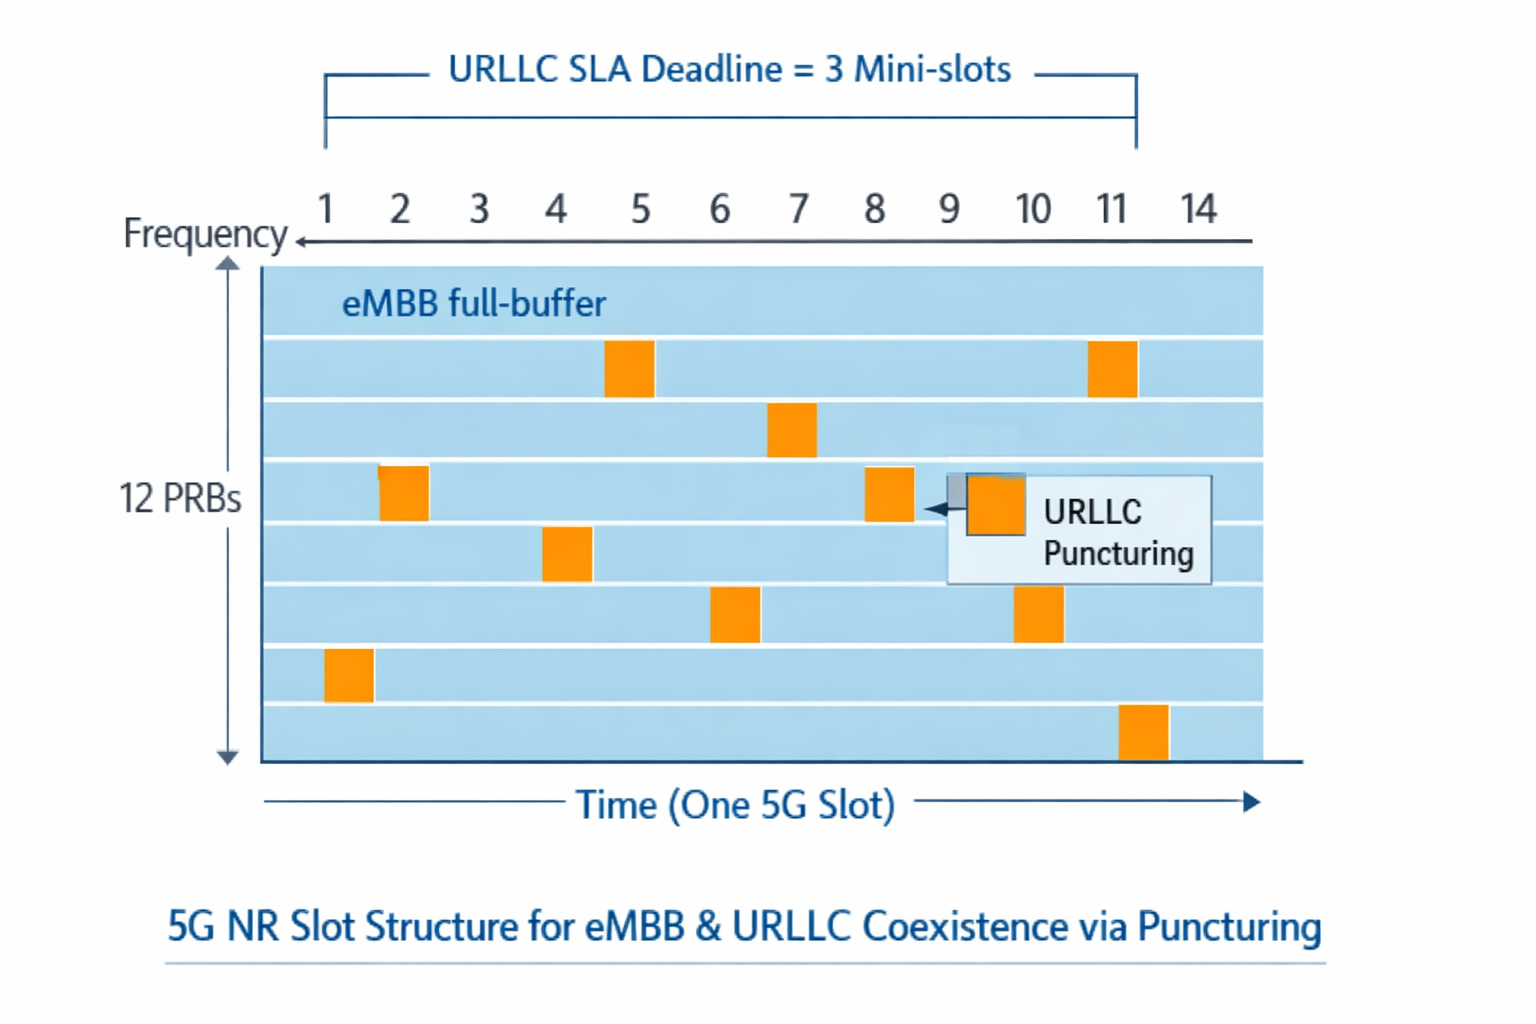
\includegraphics[width=0.9\textwidth]{eMBB与URLLC的MAC层共存结构.png}
\caption{eMBB 与 URLLC 的 MAC 层共存结构}
\label{fig:mac_coexistence}
\end{figure}

在第五代（5G）移动通信系统中，国际电信联盟（ITU）将应用场景主要划分为三大类：增强型移动宽带（eMBB）、海量机器类通信（mMTC）以及超可靠低时延通信（URLLC）。为了在统一的物理基础设施上同时支持这些具有异构需求的服务，5G New Radio（NR）引入了网络切片（Network Slicing）技术以及灵活的物理层参数集（Numerology）和帧结构设计。

eMBB 业务大多面向高速率数据传输，同时对可靠性也有一定的要求，例如分组错误率（PER）通常在 $10^{-3}$ 左右。为了获得较充分的信道编码增益、提高频谱效率，并减少频繁调度带来的控制信令开销，eMBB 通常会在较长的传输时间间隔（Transmission Time Interval, TTI）上进行调度。在 5G NR 的标准时域结构中，eMBB 的基础调度单位是时隙（Slot）。在正常循环前缀的这个条件下，一个 Slot 一般的来说包含 14 个正交频分复用（OFDM）符号。不过，Slot 的绝对时间长度可并不是固定的 1 ms，而是由灵活参数集决定的，具体来说，NR 的子载波间隔满足 $\Delta f = 2^\mu \cdot 15$ kHz这个条件就可以啦。
随着参数集索引 $\mu$ 增大，OFDM 符号持续时间与 Slot 时长近似按比例缩短。例如在 Normal CP 下，$\mu=0$（15 kHz）对应
约 1 ms Slot，而 $\mu=2$（60 kHz）和 $\mu=3$（120 kHz）时 Slot 时长分别约为 0.25 ms 和 0.125 ms\cite{ji2018, huang2022deluxe}。

和 eMBB 不太一样，URLLC 业务更多服务于工业控制、自动驾驶和远程医疗这类关键任务，它对可靠性和低时延的要求会更严格，比如 PER 要达到 $10^{-5}$，端到端时延一般也要压到 1 毫秒以内，URLLC 流量又有很强的突发性和随机性，如果数据来了以后还要等到下一个完整 Slot 边界才能拿到资源并开始发送，队列里多等的这段时间就很容易把时延推到上限外。

针对这种等待时间过长的问题，3GPP 在 5G NR 标准里加入了微时隙（Mini-slot）机制，Mini-slot 不用占满一个完整 Slot，只需要用到若干个 OFDM 符号就能完成调度，常见长度有 2、4 或 7 个符号，这样 URLLC 数据包到达基站后，就能在更细的符号边界上触发调度和传输，不必再等完整 Slot 从头开始；URLLC 要做到低时延，还需要物理层参数一起配合，比如采用 60 kHz 或 120 kHz 这类更大的子载波间隔，把单个 OFDM 符号的持续时间缩短，从而继续减少传输时延和调度等待时延。

从资源分配角度看，eMBB 和 URLLC 在底层调度粒度上不一样，这种差别会直接变成 MAC 层的调度冲突，eMBB 更适合占用连续而且时间较长的时频资源块，用来保证吞吐量和编码效率；URLLC 则更看重业务到达后能不能马上接入信道，并且在调度时通常需要更高优先级，两类业务使用资源的方式不一样，也就形成了后面资源复用和打孔调度问题的主要来源。
\begin{table}[htbp]
\centering
\small
\setlength{\tabcolsep}{4pt}
\caption{eMBB 与 URLLC 的底层差异对比}
\label{tab:embb_urllc_comparison}
\renewcommand{\arraystretch}{1.3}
\begin{tabularx}{\textwidth}{@{}>{\raggedright\arraybackslash}p{0.24\textwidth}>{\raggedright\arraybackslash}p{0.30\textwidth}>{\raggedright\arraybackslash}X@{}}
\toprule
\textbf{维度} & \textbf{eMBB} & \textbf{URLLC} \\
\midrule
调度粒度 & 完整 Slot（Normal CP 下通常 14 个 OFDM 符号，时长随 $\mu$ 缩短） & Mini-slot（符号级/微时隙级） \\
目标时延 & 大于 10 ms 可接受 & $\le 1$ ms \\
目标可靠性 & BLER $\approx 10^{-3}$ & BLER $\le 10^{-5}$ \\
流量特征 & 持续性、大负载 & 突发性、短包（Short Packet） \\
资源冲突时优先级 & 低（可被抢占或打孔） & 高（优先保障） \\
\bottomrule
\end{tabularx}
\end{table}

\subsection{打孔与叠加的物理层工作机制及理论损失模型}\label{212-ux6253ux5b54打孔ux4e0eux53e0ux52a0superpositionux7684ux7269ux7406ux5c42ux5de5ux4f5cux673aux5236}


无线电的频谱资源一直都很紧缺。要是我们像以前那样，老老实实给 URLLC 划出一块专属的正交频段（也就是正交切片），隔离效果确实好。但如果 URLLC 没数据要传，这块地空着就会白白浪费。考虑到这一点，5G NR 大都采用“动态多路复用”这种非正交的共享玩法，这种方法可以在有突发的 URLLC 数据砸过来的时候，跑去 eMBB 用户的地盘上“抢”资源。具体怎么抢呢？物理层有两招：一是“叠加”，二是“打孔”。

叠加机制指的是基站同时给 eMBB 和 URLLC 都分配发射功率，让这两路信号混在一起发出去，这其实也就是物理层常说的 NOMA（非正交多址接入）。不过这套方案看起来简单，实际上有个硬伤，那就是接收端想要把信号拆解还原出来，就得拼命指望 SIC（连续干扰消除）技术。这无疑给 eMBB 接收端添了很大堵，不只算起来极其复杂，处理时延也跟着大幅飙升。

相比之下，“打孔”机制（大家也常叫它抢占式调度）就粗暴得多。基站只要发现资源冲突了，会立刻掐断 eMBB 正在传的数据。它会把那部分冲突资源上的 eMBB 发射功率直接压到底（降到零），把地方彻底腾出来，全盘的交给 URLLC包去用。由于避免了复杂的干扰消除，打孔机制在满足 URLLC 严格时延方面表现较好，但代价是造成了 eMBB 数据包的部分损坏，并降低 eMBB 的吞吐量和链路可靠性。

至于 eMBB 数据被“打孔”后到底会受多大影响，学术界通常会用三种模型来评估。
第一种是线性损失模型。我感觉这个最好理解，就是假定 eMBB 的容量损失跟被打掉的 Mini-slot 比例是一比一挂钩的。不过在现实里，这种理想状态（比如假设信道完美且能精确预知打孔位置）往往不太成立。
第二种是凸函数损失模型。它觉得丢掉的速率是打孔比例的凸函数。说白了就是，可能只要稍微被打掉一点数据，整体性能就会出现“大跳水”。
前面这两个模型多少有点偏重理论推导，相比之下，第三种阈值损失模型就明显更接地气，更符合现在物理层信道的工程实际。如今的通信系统基本都会用上前向纠错码（FEC），相当于给数据穿了件“防弹衣”。在这个模型里，每个 eMBB 的码字 $w$ 都有一个自己能抗住的挨打极限（也就是容错上限 $C_w$）。只要 URLLC 过来“打孔”擦掉的数据量没有越过 $C_w$ 这个底线，接收端照样能把原始数据破译出来。可一旦超出了这条红线，整个码字就会直接发生彻底中断，这部分数据也就彻底凉了。有了这个阈值模型后，我们再去跑深度强化学习（DRL），状态空间的设计就有了很实在的物理底座支撑。这时候，调度器在调度的时候，眼光就不能只盯着怎么把眼前的瞬时容量拉爆了。它必须学会“察言观色”，去盯着每个频段看 eMBB 码字还能再挨几下打（感知剩余容限）。
看准了之后，再把 URLLC 数据塞到那些哪怕掉点肉也能抗住局部擦除的资源上去。这样从底层的机制上捋下来，eMBB 掉线中断的风险也就跟着大幅降下来了。


\subsection{面向网络切片的不确定性与风险敏感调度理论}\label{213-ux9762ux5411ux672aux77e5ux5230ux8fbeux7387ux7684ux9c81ux68d2ux6027ux6d4bux8bd5ux4e0eux98ceux9669ux538cux6076风险规避ux6253ux5b54ux6269ux5c55}


以前做资源分配时，大多数前辈大都喜欢套用固定的流量模型（比如假设流量按泊松或者伯努利分布来计算）。这种做法在某些特定场景下确实能算出近乎完美的调度策略，但是在真实的 5G 或者未来的 B5G 工业和车联网里，情况根本就不可能这么理想，系统里到处都是不确定性。URLLC 数据包本来就短，加上它们在什么时间、什么地点冒出来，完全是随机的。我打个比方，工业流水线上如果突然出了个故障，底下的传感器立马就会在同一秒钟把成百上千的警报砸向网络。

要是 URLLC 的突发流量一下子爆表了，远远超出了咱们系统一开始设想的分布范围（也就是常说的 OOD 场景），那些传统的“贪婪”调度算法就不管用了。这些算法平时只盯着怎么把系统的总吞吐量刷高，遇到突发情况，它们就会去“欺软怕硬”——直接把信道条件不太好的 eMBB 用户当成炮灰，把“打孔”的压力全丢给少数几条弱链路去扛。从大盘面上看，这么干确实保住了挺高的平均吞吐量。但实际上，被牺牲掉的那些 eMBB 用户早就彻底断网了，这无疑是把网络切片的公平性和 SLA（服务等级协议）完完全全的忽视了。

为了填平这个坑，现在的研究大都引入了一套叫“风险敏感”的调度思路。其实这就跟金融圈里搞投资（比如现代投资组合理论 MPT）是一个道理：在情况不明朗的时候做决定，眼光不能只死盯着能赚多少钱（期望的平均吞吐量），还得时刻防着赔本的风险（收益的波动），并给这些高风险操作加上“惩罚”。

放到 eMBB 和 URLLC 混着跑的场景里，所谓的“风险”，往细了说可以是 eMBB 吞吐量忽高忽低的方差，或者极端情况下的尾部损失（CVaR）。往实了说，也就是我这篇文章最关心的事情，别把打孔的压力全堆在少部分人身上。我在写优化目标的时候，只要给频域上的打孔负载加上一道紧箍咒，或者压住数据速率掉底的长尾风险，这个调度机制就自动带上了“避险”的基因。这么一来，基站的调度器再去抢资源时就不敢乱来了，它会老老实实地把 URLLC 的流量尽量平均摊给所有活跃的 eMBB 链路。这就能有效避免逮住一只羊薅羊毛，不让任何一个单一用户挨上超过自己容忍底线的“打孔”次数。

有了这套带着风险感知意识的理论底子后，我之后再去扩展系统的鲁棒性，或者设计新算法，心里就有行动指南了。从这些探讨也能看出来，一个真正聪明的调度模型，必须要接得住各种没见过、或者极端的流量洪峰。它不只可以死死守住 URLLC 那点严苛的时延底线，还能顺手通过这套风险管控机制，把 eMBB 切片的大盘子给稳住，保证整体的可靠和连通。












\section{深度强化学习基础}\label{22-ux6df1ux5ea6ux5f3aux5316ux5b66ux4e60ux57faux7840}



\subsection{MDP 的标准数学定义}\label{221-mdp的标准数学定义}

\begin{figure}[H]
\centering
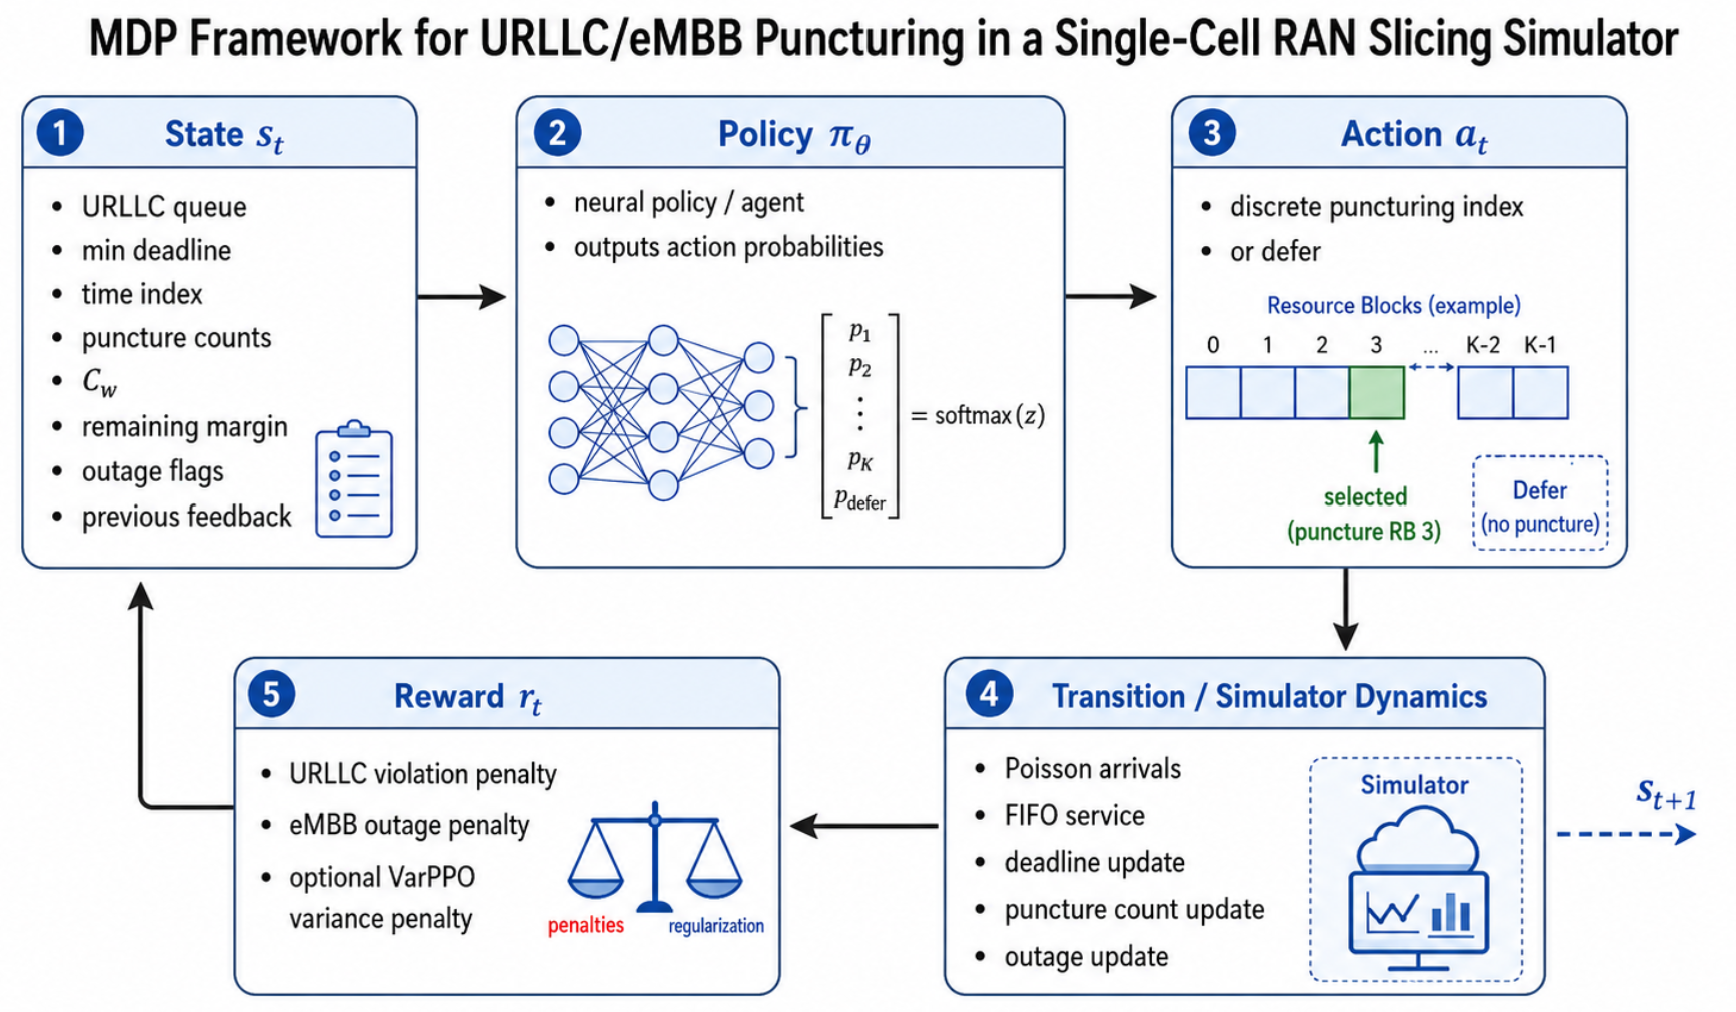
\includegraphics[width=0.9\textwidth]{MDP建模框架.png}
\caption{MDP 建模框架}
\label{fig:mdp_framework}
\end{figure}

深度强化学习的数学基础是马尔可夫决策过程（Markov Decision Process, MDP）。在通信网络的资源调度问题中，通常将其建模为一个离散时间随机控制过程（Discrete Time Stochastic Control Process）。一个标准的 MDP 被形式化定义为一个五元组 $\mathcal{M} = (\mathcal{S}, \mathcal{A}, \mathcal{P}, \mathcal{R}, \gamma)$，其中：

\begin{itemize}
\item
$\mathcal{S}$ 表示状态空间（State Space），$s_t \in \mathcal{S}$ 表示智能体在时刻 $t$ 观测到的环境状态，通常包括与当前决策有关的主要特征；
\item
$\mathcal{A}$ 表示动作空间（Action Space），$a_t \in \mathcal{A}$ 表示智能体在状态 $s_t$ 下可以选择并执行的动作；
\item
$\mathcal{P}(s_{t+1} \mid s_t, a_t)$ 表示状态转移概率，主要说明智能体执行动作 $a_t$ 之后，系统有多大可能从当前状态 $s_t$ 走到下一状态 $s_{t+1}$，这个变化过程满足马尔可夫性质，也就是说下一状态只和当前状态、当前动作有关，不用再把更早的历史过程都算进去；
\item
$\mathcal{R}(s_t, a_t)$ 表示即时奖励函数，用来评价智能体在状态 $s_t$ 下执行动作 $a_t$ 后拿到的反馈，奖励值越高，一般说明这个动作在当前状态下带来的效果越好，后续调整策略时也会把它作为重要依据；
\item
$\gamma \in [0, 1)$ 表示折扣因子，用来调节当前奖励和未来奖励之间的比重，$\gamma$ 越接近 1，智能体就会更看重长期收益，$\gamma$ 越小，它就会更关注眼前能够拿到的即时奖励。
\end{itemize}

在上述设定下，智能体的目标是找到一个最优策略 $\pi^*(a \mid s)$，使这个所谓的策略在长期交互过程中获得尽可能大的期望累积折扣回报，目标函数可以写为：
\begin{equation}
J(\pi) = \mathbb{E}{\pi} \left[ \sum{t=0}^{\infty} \gamma^t \mathcal{R}(s_t, a_t) \right].
\label{eq}
\end{equation}

其中，状态价值函数 $V^\pi(s)$ 表示智能体从状态 $s$ 出发，并按照策略 $\pi$ 持续行动时，未来能够获得的期望累积回报；动作价值函数 $Q^\pi(s, a)$ 则表示智能体在状态 $s$ 下先执行动作 $a$，之后再按照策略 $\pi$ 行动时，未来能够获得的期望累积回报。两类价值函数可以通过 Bellman 方程建立递推关系，这也为后续深度强化学习算法中的参数更新提供了基础，例如我后续基于 Actor-Critic 架构的 PPO 算法，就会利用价值估计来辅助策略网络的训练。


%（注：关于状态向量的具体数学表达、奖励函数的完整数学公式以及环境状态转移的详细机制，将在第三章“系统建模与算法设计”中展开深入论述。）








\subsection{从 Q-Learning 到 DQN：基于值函数方法的演进与局限性}\label{222-从-q-learning-到-dqn基于值函数方法的进展与瓶颈}
Q-Learning~\cite{watkins1992} 是一种经典的无模型（Model-free）强化学习算法。这里的“无模型”并不是说算法没有数学表达，而是说智能体在做决策前，不需要提前知道环境的状态转移概率或具体的动态方程。我就以无线资源调度为例，调度器不必事先掌握无线信道衰落的精确马尔可夫转移矩阵，也不需要知道业务到达过程的泊松分布参数，而是可以通过和环境不断交互、试错，逐步学到较优的决策方式。Q-Learning 的核心思想是利用时序差分（Temporal Difference, TD）方法，对动作价值函数进行反复更新，从而逐渐一步一步的来逼近最优动作价值函数。$Q^*(s, a)$：
\begin{equation}
Q(s_t, a_t) \leftarrow Q(s_t, a_t) + \alpha \left[ r_t + \gamma \max_{a'} Q(s_{t+1}, a') - Q(s_t, a_t) \right].
\label{eq:q_learning_update}
\end{equation}
在该更新规则中，Q-Learning 是一种异策略（Off-policy）算法，即智能体用于更新价值网络的数据，不必严格由当前的调度策略产生，它可以利用历史探索产生的数据进行学习。然而，传统 Q-Learning 以查找表（Q-table）的形式存储所有“状态-动作”对的 Q 值。在本文的 5G RAN 切片场景中，状态空间包含了 URLLC 队列长度、各个频段上 eMBB 码字的剩余打孔次数等特征的组合。面对如此高维的特征，传统 Q 表会遭遇“维数爆炸（Curse of Dimensionality）”，导致其在物理内存存储与穷举查询上均不可行。

为克服这一理论瓶颈，深度 Q 网络（Deep Q-Network, DQN）~\cite{fan2020} 采用深度神经网络 $Q(s, a; \theta)$ 来拟合近似传统的 Q 表，并通过引入两项关键技术来解决神经网络在强化学习中容易发散的问题：
\begin{itemize}
\item 经验回放（Experience Replay）： 智能体将历史上经历过的状态转移元组（包含当前状态、动作、奖励、下一状态）存入一个回放缓冲区中。训练时，从中进行随机小批量采样。在通信系统中，连续时间步的信道状态和队列状态往往具有高度的时间相关性，直接顺序训练会导致网络严重过拟合。经验回放机制打破了样本间的时序相关性，使训练数据更趋近于独立同分布（i.i.d），从而提升了训练效率。
\item 目标网络（Target Network）： 在强化学习中，上述公式中的目标值（即 $r_t + \gamma \max_{a'} Q$）本身也是由神经网络预测产生的，这种“用自己的估计值来更新自己”的机制被称为自举（Bootstrapping）。如果频繁更新，会导致目标值剧烈震荡进而发散。
DQN 这种方法可以造出一个与主网络结构相同但参数滞后更新的“目标网络”，专门用于计算目标值，最终来稳定网络训练。
\end{itemize}

基于值函数的方法在混合流量切片问题中存在一些瓶颈。DQN 虽然已经在很多任务中取得了较好的效果，但在处理本文关注的 URLLC 与 eMBB 混合复用问题时，仍然会有一些不容易忽视的限制。一方面，我需要区分本文采用的简化动作空间和真实系统中更复杂的 URLLC 调度动作空间。在本文构建的单小区抽象环境中，若每个 Mini-slot 只需要从 $K$ 个频域资源中选择一个打孔位置，那么动作数量大致只有 $K$ 个，若再考虑“不服务”或空动作，也只是顶多增加一个动作。从这个角度看，DQN 在形式上仿佛并不是完全不能使用。真正影响 DQN 扩展能力的，是更接近实际系统的组合动作空间（Combinatorial Action Space），例如当 URLLC 突发包较大时，一次调度可能需要同时选择 $m$ 个频段，或者多个 PRB 组进行打孔，此时可选动作数量会增加到 $\binom{K}{m}$，这样一来，Q 值枚举、动作探索和样本覆盖都会变得越来越困难。另一方面，Q-Learning 这类方法在更新过程中通常会用到 $\max$ 操作，如前文公式所示。在泊松到达、无线信道衰落等随机性较强的通信环境中，$\max$ 操作容易带来最大化偏差（Maximization Bias），也就是环境噪声和随机波动可能会被 $\max$ 算子进一步放大，使模型对某些动作的 Q 值产生持续偏高的估计。
与此同时，DQN 依赖经验回放和滞后更新的目标网络来稳定训练；在高频 Mini-slot 调度中，历史样本分布与当前队列、信道和打孔状态可能快速偏离，目标网络滞后也可能削弱智能体对突发流量变化的在线适应能力。

鉴于基于值函数的 DQN 在组合式离散调度中可能面临动作枚举爆炸、最大化偏差和动态分布滞后等问题，研究者们也曾尝试转向基于策略搜索的基础策略梯度方法（Vanilla Policy Gradient, VPG）。然而，VPG 对学习率和采样方差高度敏感，训练过程中容易出现震荡甚至策略性能退化。
基于上述考虑，本文的实现没有沿用 DQN 或基础 VPG，而是采用近端策略优化（Proximal Policy Optimization, PPO）算法。PPO 通过裁剪代理目标（Clipped Surrogate Objective）限制新旧策略之间的概率比变化，在无需显式二阶近似运算的前提下实现近似信赖域更新，工程上通常比基础策略梯度更稳定，适合用于本文这种离散抢占决策空间下的在线试错训练。但需要指出的是，PPO 并不保证在所有随机环境和有限训练步数下都单调提升；本文后续实验仅基于当前仿真环境和训练配置评价其经验性能。









\subsection{策略梯度定理、PPO 的裁剪目标与 GAE 优势估计}\label{223-ux7b56ux7565ux68afux5ea6ux5b9aux7406ppo-ux7684ux88c1ux526aux76eeux6807ux4e0e-gae-ux4f18ux52bfux4f30ux8ba1}

在动态无线网络的资源切片和调度问题中，URLLC 业务到达比较突然，时延要求又很低，传统启发式算法很难在微秒级 mini-slot 时间内算出足够合适的抢占方案，本文因此引入基于策略梯度（Policy Gradient）的深度强化学习方法，为混合业务场景中的智能抢占（Preemption）调度提供算法依据。策略梯度方法不再先估计每个动作的固定价值，而是直接优化参数化策略 $\pi_\theta(a \mid s)$，让策略逐步提高高回报动作的选择概率。根据策略梯度定理~\cite{sutton1999}，目标函数 $J(\pi_\theta)$ 对策略参数 $\theta$ 的梯度可以写成
\begin{equation}
\nabla_\theta J(\pi_\theta)
=
\mathbb{E}_{\pi_\theta}
\left[
\nabla_\theta \log \pi_\theta(a_t \mid s_t)\cdot A^\pi(s_t,a_t)
\right],
\label{eq:policy_gradient}
\end{equation}
其中，$A^\pi(s_t,a_t)=Q^\pi(s_t,a_t)-V^\pi(s_t)$ 表示优势函数（Advantage Function），它衡量的是在状态 $s_t$ 下选择动作 $a_t$，相对于该状态平均收益能多带来多少价值。直接依靠采样来估计梯度时，结果往往会有较大波动，所以常用的策略梯度算法会采用 Actor-Critic 架构：Actor 网络负责给出并更新策略，Critic 网络估计状态价值函数 $V^\pi(s_t)$，再把价值判断反馈给 Actor，帮助它判断更新方向。

传统策略梯度方法更新参数时，很难把步长控制得刚好合适，更新太大可能会让策略性能突然下降，甚至出现策略崩溃（Policy Collapse），更新太小又会拖慢收敛速度。信赖域策略优化（TRPO）用 KL 散度约束来限制新旧策略之间的差距，不过它需要二阶优化和矩阵相关计算，实际开销比较高。近端策略优化（Proximal Policy Optimization, PPO）采用更轻量的一阶近似思路，通过裁剪替代目标函数（Clipped Surrogate Objective）来约束策略变化，不需要显式求解复杂的约束优化问题，也能得到近似信赖域更新的效果，其目标函数为
\begin{equation}
L^{\mathrm{CLIP}}(\theta)
=
\mathbb{E}_t
\left[
\min\!\Big(
r_t(\theta)\hat{A}_t,\,
\mathrm{clip}\big(r_t(\theta),1-\epsilon,1+\epsilon\big)\hat{A}_t
\Big)
\right],
\label{eq:ppo_clip_objective}
\end{equation}
其中，概率比 \(r_t(\theta)=\pi_\theta(a_t \mid s_t)/\pi_{\theta_{\mathrm{old}}}(a_t \mid s_t)\) 用来表示更新前后同一动作概率的变化程度，裁剪超参数 $\epsilon$ 则控制一次更新能走多远。当概率比超过 $[1-\epsilon,1+\epsilon]$ 这个区间，而且这种变化还会继续放大目标函数时，PPO 会把对应项限制在边界内，避免策略一下子偏向过于极端的动作，从而让训练过程更稳定。

为了让 Actor 更新时的梯度波动小一些，训练过程也更稳一些，本文在 Stable-Baselines3 强化学习框架里同时使用 PPO 和广义优势估计（Generalized Advantage Estimation, GAE-$\lambda$）机制，GAE 会加入衰减参数 $\lambda_{\mathrm{GAE}}$，把不同时间步上的时序差分（TD）误差按照指数权重累加起来，这样优势估计不会太偏，也不会因为方差过大而剧烈抖动；结合本文分布外（Out-of-Distribution, OOD）URLLC 到达率鲁棒性测试场景来看，例如到达率 $\lambda \in [0.2,1.5]$ 发生变化时，PPO 的裁剪机制能把过大的策略更新压下来，GAE 又能借助价值网络把长期收益估计得更平滑，两者配合后，可以给随机流量较强的训练环境提供更稳定的算法基础。

整体来看，在本文的切片资源分配模型里，PPO 主要用来处理离散抢占决策，GAE 主要用来降低优势估计的方差并让策略训练更平稳；本文还加入了面向频域打孔负载均衡的定制化奖励函数，让智能体在减少 URLLC 违约和控制 eMBB 中断之间做取舍，同时尽量避免物理层打孔长期堆在少数子载波上，这些内容也为后面的资源切片优化实验提供了理论和工程上的基础。







\section{本章小结}


本章主要从通信机制和深度强化学习两个角度，整理了 5G RAN 混合业务切片资源分配中会用到的基础知识，为后续系统建模和算法设计做了铺垫。

在通信机制层面，一方面，本章对比了 eMBB 与 URLLC 在物理层和 MAC 层上的主要差异，eMBB 通常把完整 Slot 当作调度粒度，在 Normal CP 条件下，每个 Slot 一般有 14 个 OFDM 符号，不过 Slot 的实际时长由 NR Numerology 决定，并且会随着 $\mu$ 增大而变短；URLLC 则更多依靠 Mini-slot 机制和更大的子载波间隔，在符号级时间尺度上更快触发调度，用来满足端到端时延不超过 1 ms、可靠性达到 BLER $\leq 10^{-5}$ 的要求。另一方面，本章也整理了动态频谱复用中的打孔（Puncturing）和叠加（Superposition）两种物理层机制，并重点解释了阈值损失模型（Threshold Model）的含义，也就是把 eMBB 码字的容错上限 $C_w$ 放进状态特征里，让智能体能够感知链路的脆弱程度，这为后续“容忍度感知抢占决策”的调度建模提供了物理层依据；针对真实网络中 URLLC 到达率很难提前确定的问题，本章还引入了风险敏感（Risk-Sensitive）调度思想，通过在优化目标里约束频域打孔负载分布或条件风险价值（CVaR），说明风险规避机制可以为降低 eMBB 切片用户中断风险、改善服务等级协议（SLA）公平性提供参考。

在深度强化学习基础层面，本章把切片动态调度问题写成马尔可夫决策过程（MDP）五元组 $\mathcal{M} = (\mathcal{S}, \mathcal{A}, \mathcal{P}, \mathcal{R}, \gamma)$，并说明智能体需要尽量最大化期望累积折扣回报；之后，本章分析了传统 Q-Learning 与 DQN 在高维状态表示、组合动作扩展、最大化偏差和动态分布滞后等方面的不足，也说明基础策略梯度方法（VPG）在训练时容易出现波动，因此有必要使用更稳定的策略优化方法。本章还说明了近端策略优化（PPO）的裁剪代理目标函数 $L^{\mathrm{CLIP}}(\theta)$ 与广义优势估计（GAE-$\lambda$）机制的基本原理，PPO 通过概率比裁剪来限制策略更新幅度，让训练过程更接近稳定的信赖域更新，GAE-$\lambda$ 则把多步 TD 误差按照指数权重累加起来，在估计偏差和估计方差之间做折中。

由以上分析可以看出，PPO 与 GAE-$\lambda$ 结合后的 Actor-Critic 架构，比较适合处理本文中的离散抢占决策空间、混合业务奖励分布以及 OOD 鲁棒性评估问题。本章完成的理论梳理和技术可行性分析，也为第三章构建通信队列动力学模型、定义 MDP 状态与动作空间，以及推导融合风险规避指标的多目标奖励函数提供了基础。

\chapter{系统建模与算法设计}\label{ux7b2cux4e09ux7ae0-ux7cfbux7edfux5efaux6a21ux4e0eux7b97ux6cd5ux8bbeux8ba1}


\section{系统模型与场景描述}\label{31-ux7cfbux7edfux6a21ux578bux4e0eux573aux666fux63cfux8ff0}

\begin{figure}[H]
\centering
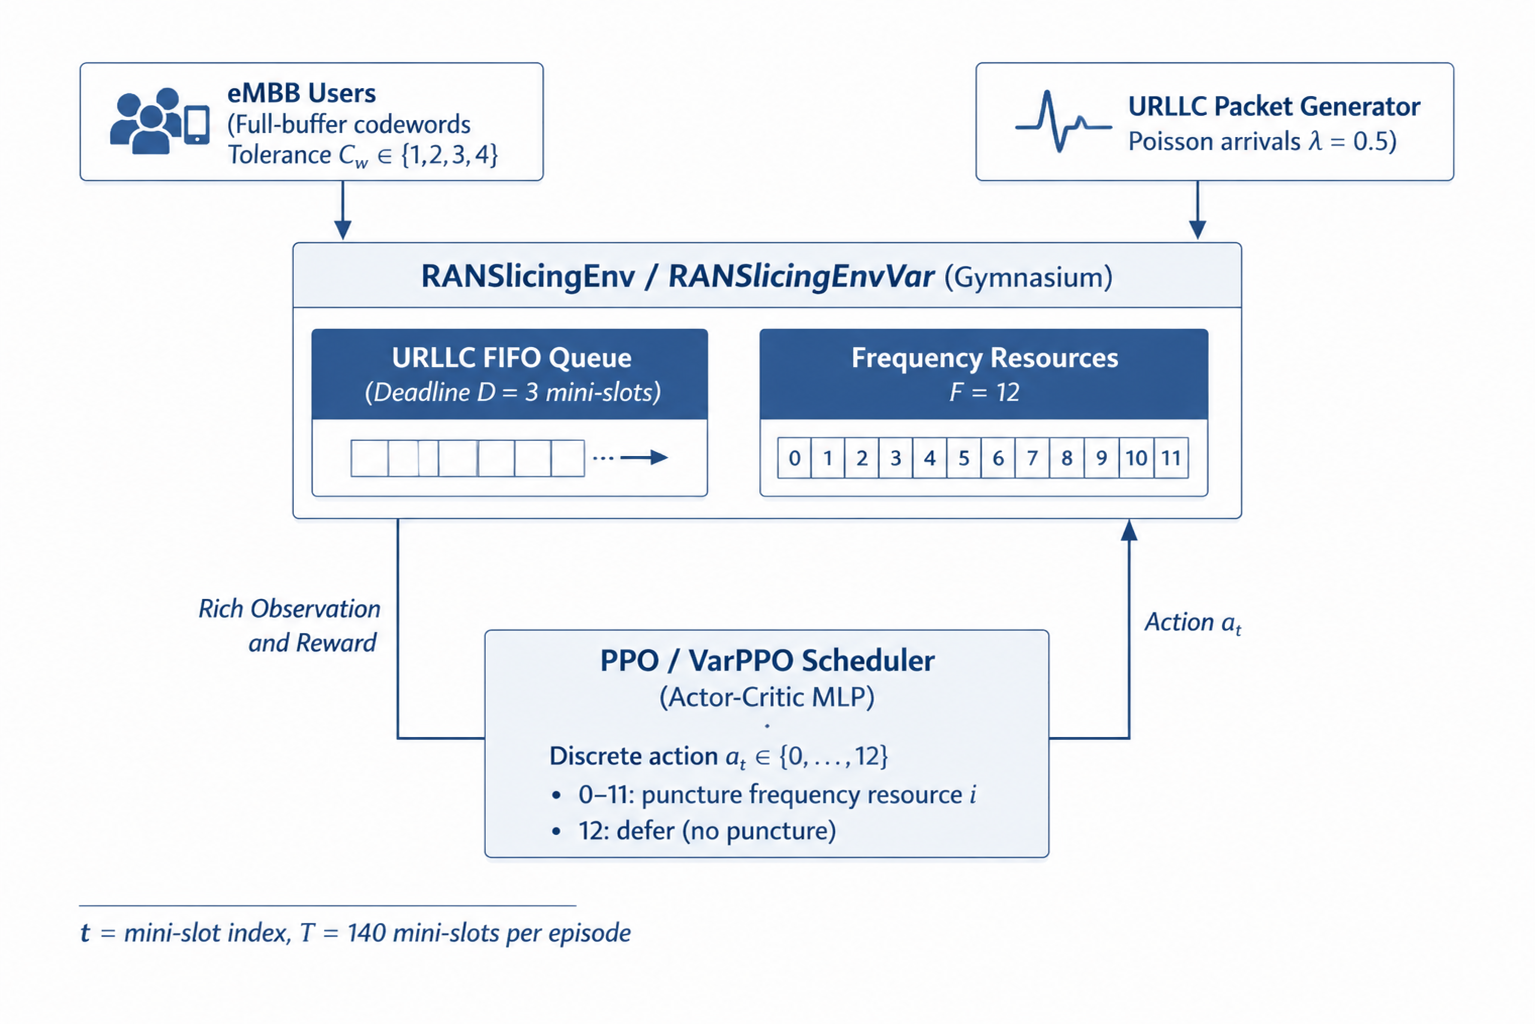
\includegraphics[width=0.9\textwidth]{Gymnasium仿真环境系统模型.png}
\caption{Gymnasium 仿真环境系统模型}
\label{fig:gymnasium_system_model}
\end{figure}

\subsection{网络拓扑与时域结构}\label{311-ux7f51ux7edcux62d3ux6251ux4e0eux65f6ux57dfux7ed3ux6784}

本文把系统模型实现成一个基于 Gymnasium 的离散时间仿真环境，时域结构主要参考 5G NR 的标准帧结构，同时也考虑到无线信道在一段相干时间内变化较小的特点，因此在仿真中采用 Slot 和 Mini-slot 两级时间划分：

\begin{itemize}
\item
  \textbf{Slot（时隙）层}：单次回合（Episode）的时间范围对应无线信道的一段相干时间，并假定信道在这段时间内基本保持不变。仿真中把相干时间设为 10 ms，每个 Slot 的持续时间设为 1 ms\cite{saggese2021}，这样一来，一个回合正好包含 10 个 Slot，也和 5G NR 中 10 ms 无线电帧、10 个 1 ms 子帧的结构相对应\cite{alsenwi2021}。从物理意义看，根据 \(T_c \approx 1/f_d\) 可以知道，10 ms 的相干时间大约对应 100 Hz 的多普勒频移；如果中心载频取 C-Band 中常见的 3.5 GHz，那么对应的移动速度约为 \(30~\mathrm{km/h}\)，可以近似表示城市道路中的低速移动场景。因此，系统一共包含 \(\Sigma = 10\) 个时隙（Slot），每个 Slot 在频域上都会对应一组在时隙边界处分配给 eMBB 用户的码字。
\item
  \textbf{Mini-slot（微时隙）层}：URLLC 流量对时延要求很高，如果只按完整 Slot 调度，反应速度往往不够，因此每个 1 ms 的 Slot 会继续划分成 \(M = 14\) 个 Mini-slot。这个设置对应 5G NR 物理层中每个 1 ms 时隙包含 14 个 OFDM 符号的特点\cite{alqwider2024}。在本文的仿真里，Mini-slot 是 PPO 智能体执行调度和处理 URLLC 突发流量的最小时间步，智能体会在这个粒度上做出抢占决策（Preemption Decision），而这个决策落到物理层后，就表现为对相应 eMBB 码字产生打孔效应（Puncturing Effect）。
\end{itemize}

单次回合（Episode）的总时步数由相干时间内的总 Mini-slot 数量决定，即 \(T = \Sigma \times M = 10 \times 14 = 140\)。时步索引为 \(t \in \{0, 1, \ldots, T-1\}\)，当前所属的 Slot 索引由整除关系 \(\text{slot\_idx}(t) = \left\lfloor t/M \right\rfloor\) 确定。
在频域上，系统带宽被划分为 \(F = 12\) 个正交频率资源（仿真中对频域资源的抽象离散化单元，每个频率资源对应一路独立的eMBB码字），它们与时域结构共同构成了供 eMBB 和 URLLC 服务复用的时频资源网格。

\subsection{eMBB 码字容忍度模型与完美 CSI 上界假设}\label{312-embb-ux7801ux5b57ux5bb9ux5fcdux5ea6ux6a21ux578b}

本模型对物理层链路自适应进行了适度抽象，采用打孔抗性（Puncturing Resilience）或容忍度上界（Tolerance Upper-bound）替代复杂的底层信道编码与解码器级仿真。原基线文献通常仅考虑简化的 \(\{0, 1\}\) 容忍度类\cite{saggese2021}；为了配合本研究中后续引入的频域打孔负载均衡机制\cite{alsenwi2021}并提供更细粒度的风险梯度，本文将容忍度范围扩展为多个整数等级。

需要说明的是，本文中的 eMBB 码字可靠性裕度 \(C_w\)，不是真实 gNB 在 HARQ 反馈返回前就能完全确定的物理层隐藏量。为了把讨论重点放到离散抢占决策和频域打孔负载均衡机制本身，本文在第三章及后续仿真实验中采用完美信道状态信息（Perfect CSI）假设，也就是环境会在每个 Slot 开始时，把当前 eMBB 码字的理想可靠性裕度 \(C_w\) 提供给智能体，这个值可以看作 oracle-assisted 的码字容忍度上界；换句话说，本文结果主要刻画的是理想信道可观测条件下 VarPPO 能达到的理论性能上界，并不表示真实 5G gNB 在存在 CQI 反馈时延、MCS 选择误差和 HARQ 延迟时，仍然能精确得到 \(C_w\)。

在每个 Slot 开始时（也就是 \(\text{slot\_idx}(t)\) 发生变化时），环境会为每个子载波 \(f \in \{0,1,\ldots,F-1\}\) 独立抽取一个取值范围更宽的整数容忍度，即
\begin{equation}
C_{w,f} \equiv \tau_f \sim \text{Uniform}\{1, 2, 3, 4\}, \quad \forall f.
\label{eq:codeword_tolerance_distribution}
\end{equation}
\(\tau_f\) 与 \(C_{w,f}\) 在本文仿真中等价，均表示子载波 \(f\) 上的 eMBB 码字在同一 Slot 内能够承受的最大打孔次数。与此同时，系统会维护每个子载波的累积打孔计数 \(p_f(t)\) 和码字中断状态 \(O_f(t) \in \{0, 1\}\)。一旦 \(p_f(t) > C_{w,f}\)，码字即发生中断。


\section{队列动力学模型}\label{32-ux961fux5217ux52a8ux529bux5b66ux6a21ux578b}

\subsection{URLLC 到达过程与时延预算模型}\label{321-urllc-ux5230ux8fbeux8fc7ux7a0bux4e0eux65f6ux5ef6ux9884ux7b97ux6a21ux578b}

URLLC 数据包的到达过程用参数 \(\lambda\) 的泊松过程表示，也就是时步 \(t\) 的到达量满足 \(A(t) \sim \text{Poisson}(\lambda)\)，基础训练时取 \(\lambda = 0.5\)；为了看算法遇到越界到达率（Out-of-Distribution Arrival Rates）以后还能不能保持较好的泛化能力和稳定性，本章对 URLLC 的时延容忍度重新做了收紧处理，母本基线模型把 \(1\,\text{ms}\) 的时隙分成 \(14\) 个 Mini-slot，排队时延上限给到 \(7\) 个 Mini-slot（约 \(0.5\,\text{ms}\)），但按 \(3\text{GPP}\) 规范来看，URLLC 服务的端到端（E2E）时延上限只有 \(1\,\text{ms}\)，这 \(1\,\text{ms}\) 还要留给传播延迟、传输延迟、排队延迟以及软硬件处理延迟\cite{truong2026}；实际系统里，基带处理过程，比如编码和解码，一般会占用 \(3\) 个以上的 OFDM 符号时间\cite{esswie2018}，如果基站在排队调度阶段就用了 \(0.5\,\text{ms}\)，后面整体 E2E 时延超过要求的可能性会明显变大。

为了让模型更接近 \(5\text{G NR}\) 物理层的超低时延要求，本章把每个新到达数据包的初始剩余排队时限（Remaining Deadline）改为 \(d_{\text{init}} = D = 3\) 个 Mini-slot（约 \(0.21\,\text{ms}\)），新包仍然按先进先出（FIFO）顺序进入等待队列 \(\mathcal{Q}(t)\)；这样做可以给后面的空口传输和可能发生的重传留出一定时间，但突发流量一来，调度器能用来缓冲 eMBB 资源被抢占影响的窗口也会变小。

需要特别说明的是，为确保性能对比评估的绝对公平性，本研究并未直接引用基线文献中 $D=7$ 时的实验数据。所有的基线算法（包括原始的 PPO 算法与传统的固定规则分配算法）均在本章构建的 $D=3$ 这一相同严苛的马尔可夫决策环境约束下进行了重新评估与测试。所有算法在同等紧迫的时延压力下竞争资源，从而客观、真实地反映了本文所提算法在鲁棒性和 eMBB 中断率控制上的相对优势。









\subsection{队列更新方程}\label{322-ux961fux5217ux66f4ux65b0ux65b9ux7a0b}

队列中每个数据包 \(k\) 携带其剩余时限 \(d_k(t) \in \mathbb{Z}^+\)。智能体的动作空间为 \(\{0, 1, \dots, F\}\)，其中在时步 \(t\) 执行动作 \(a_t < F\) 表示选择对应子载波传输，\(a_t = F\) 表示暂缓（Defer）\cite{saggese2021}。系统按以下顺序更新队列状态：

\begin{enumerate}
\def\labelenumi{\arabic{enumi}.}
\item
  到达（Arrival）：向队列尾部追加 \(A(t)\) 个初始剩余时限为 \(D\) 的数据包，即 \(\mathcal{Q}(t) \leftarrow \mathcal{Q}(t) \cup \{D\}^{A(t)}\)。
\item
  服务（Service）：若队列非空且 \(a_t < F\)（即未选择 Defer 动作），则从队列头部弹出一个包进行服务（每步至多服务一个包），即当 \(\mathcal{Q}(t) \neq \emptyset\) 且 \(a_t < F\) 时执行 \(\text{popleft}(\mathcal{Q}(t))\)。
\item
  时限递减与违约统计（Deadline Update \& Violation）：对队列中所有剩余包的时限递减，即 \(d_k \leftarrow d_k - 1, \forall k \in \mathcal{Q}(t)\)，并统计违约数量 \(V(t)=\left|\{k \in \mathcal{Q}(t) : d_k \leq 0\}\right|\)。
\end{enumerate}

时限耗尽的包（\(d_k \leq 0\)）将被从队列中移除，并计入 URLLC 违约计数，不再保留，即 \(\mathcal{Q}(t+1) = \{k \in \mathcal{Q}(t) : d_k > 0\}\)。
因此，队列长度的动态更新可以写成闭式：
\begin{equation}
|\mathcal{Q}(t+1)| = |\mathcal{Q}(t)| + A(t) - \mathbb{1}[a_t < F \wedge \mathcal{Q}(t) \neq \emptyset] - V(t).
\label{eq:queue_length_update}
\end{equation}
综上，上述闭式更新关系刻画了 URLLC 缓冲队列的马尔可夫动态守恒。系统在 \(t+1\) 状态的队列长度，由当前队列积压、泊松到达增量、有效服务离队（受控于动作指示函数）以及超时违约清理四项共同决定。





\section{MDP 核心要素的数学定义}\label{33-mdp-ux6838ux5fc3ux8981ux7d20ux7684ux6570ux5b66ux5b9aux4e49}

\subsection{容忍度感知观测空间设计}\label{331-ux72b6ux6009ux7a7aux95f4-mathcals-ux4e0e-tolerance-aware-observation}

紧凑的 \texttt{minimal} 观测用于兼容旧实验设定，其形式为
\begin{equation}
\mathbf{o}^{\mathrm{min}}_t
=
\bigl[\tilde{q}(t),\tilde{d}_{\min}(t),
\tilde{p}_0(t),\ldots,\tilde{p}_{F-1}(t)\bigr]^\top
\in \mathbb{R}^{2+F}.
\label{eq:minimal_observation}
\end{equation}
在默认 \(F=12\) 时，该观测维度为 14。

\texttt{rich} 观测则进一步加入时延、时间位置和 Perfect-CSI 可靠性裕度信息，可写为
\begin{equation}
\begin{aligned}
\mathbf{o}^{\mathrm{rich}}_t =
\bigl[
&\tilde{q}(t),\tilde{d}_{\min}(t),
\mathbf{h}_D(t),
\tilde{s}(t),\tilde{m}(t),\tilde{r}(t),\\
&\tilde{\mathbf{p}}(t),
\tilde{\mathbf{C}}_w(t),
\tilde{\mathbf{g}}(t),
\mathbf{O}(t),
\tilde{A}_{t-1},\tilde{S}_{t-1},\tilde{V}_{t-1},\tilde{E}_{t-1}
\bigr]^\top ,
\end{aligned}
\label{eq:rich_observation}
\end{equation}
其中 \(\mathbf{h}_D(t)\) 为 URLLC 剩余时限直方图，\(\tilde{s}(t)\)、\(\tilde{m}(t)\) 和 \(\tilde{r}(t)\) 分别表示当前 slot 索引、当前 slot 内 mini-slot 索引以及当前 slot 内剩余 mini-slot 数的归一化值；\(\tilde{\mathbf{p}}(t)\) 为各子载波累计打孔次数；\(\tilde{\mathbf{C}}_w(t)\) 为完美 CSI 假设下各 eMBB 码字的理想可靠性裕度；\(\tilde{\mathbf{g}}(t)=\mathrm{clip}((\mathbf{C}_w(t)-\mathbf{p}(t))/C_{\max},-1,1)\) 为归一化剩余裕度；\(\mathbf{O}(t)\) 为各码字中断标志；最后四项表示上一时步的到达包数、成功服务包数、URLLC 违约数和 eMBB 中断数。默认 \(D=3,F=12\) 时，\texttt{rich} 观测维度为
\(2+D+3+4F+4 = 2+3+3+48+4 = 60\)。

本文这里使用的是完美 CSI 支持的 oracle-assisted reliability margin，这一设定能让状态转移保持为标准的 tolerance-aware MDP，也便于评估所提策略在理想可观测条件下的性能上界。转到真实系统时，\(C_w\) 只能通过 CSI、CQI/MCS、BLER 预测、链路自适应、HARQ ACK/NACK 以及译码器反馈来间接估计，而且会受到反馈时延和估计误差影响；此时问题还需要进一步扩展为含有延迟观测和状态噪声的 POMDP 或鲁棒 MDP。本文把这一方向放在后续工程化研究中讨论，当前仿真结果不再混入非理想 CSI 误差。

从通信建模角度看，\(\mathbf{o}^{\mathrm{rich}}_t\) 并不是把底层译码器状态直接交给智能体，而是把 eMBB 码字的容忍度上界、当前累计打孔计数和剩余可靠性裕度，转换成智能体能够观测到的归一化状态特征；这种设计能让强化学习策略在 MAC 层执行抢占决策时，感知到物理层打孔效应带来的风险变化，同时也让状态向量在数学形式上保持一致。

状态空间的形式化定义为：\(\mathcal{S} = \mathbb{R}^{60}\)，即由 60 个实值观测分量构成的连续状态空间。







\subsection{动作空间 \texorpdfstring{$\mathcal{A}$}{A} 与抢占语义}\label{332-ux52a8ux4f5cux7a7aux95f4-mathcala-ux4e0eux6253ux5b54ux8bedux4e49}

动作空间为离散整数空间 \(\mathcal{A} = \{0, 1, 2, \ldots, F\} = \{0, 1, \ldots, 12\}\)。其中动作索引 $0$ 至 $F-1$ 分别对应在 $F$ 个子载波上执行抢占调度，动作索引 $F$ 对应暂缓执行（Defer）。物理层的打孔仅作为该抢占决策的执行后果计入 \(p_f(t)\) 和 \(O_f(t)\)。

各动作的语义如下：

\begin{equation}
a_t =
\begin{cases}
f \in \{0,\ldots,F-1\}, & \text{对子载波 } f \text{ 执行抢占调度，服务一个 URLLC 包}, \\
F = 12, & \text{Defer：暂缓抢占，不服务任何 URLLC 包}.
\end{cases}
\label{eq:action_semantics}
\end{equation}
动作 \(a_t = f < F\) 的执行逻辑可形式化为：若 \(\mathcal{Q}(t) \neq \emptyset\) 且 \(a_t = f\)，则弹出队列头部数据包，并对子载波 \(f\) 记录一次由抢占导致的物理层打孔计数，即 \(p_f(t) \leftarrow p_f(t) + 1\)。
若此时累积打孔次数超过该子载波本 Slot 的 eMBB 码字理想容忍度 \(C_w\)，且该码字尚未被标记为中断，则触发 eMBB 码字中断事件：
\begin{equation}
O_f(t) =
\begin{cases}
1, & \text{若 } p_f(t) > C_{w,f}(t) \text{ 且 } O_f(t-1) = 0, \\
O_f(t-1), & \text{否则}.
\end{cases}
\label{eq:embb_outage_state}
\end{equation}
每步的 eMBB 新增中断计数为
\begin{equation}
E(t) = \sum_{f=0}^{F-1} \mathbb{1}\!\left[O_f \text{ 在时步 } t \text{ 首次被置为 1}\right] \in \{0, 1\}.
\label{eq:embb_new_outage_count}
\end{equation}
由于每个时步最多只会打孔一个子载波，所以有 \(E(t) \in \{0, 1\}\)。

需要特别指出的是，在 5G NR 物理层中，URLLC 对 eMBB 的打孔（Puncturing）机制，本质上是基于资源粒子（RE）或子载波粒度的硬性抢占（Hard Preemption），不是非正交多址（NOMA）那类连续功率叠加；所以，基站在频域上的调度决策具有严格的正交性和互斥性，每个子载波要么被完全占用，要么不被占用。

这个物理约束决定了强化学习动作空间需要采用离散形式。如果采用连续控制中的高斯策略（Gaussian Policy），智能体输出的连续动作（如 $a_t = 4.7$）还要通过取整才能映射到具体子载波（如第 5 号载波），但取整操作（如 Floor/Round）在大多数位置不可导，或者梯度为零，无法给 Actor 网络提供有效的策略梯度信号，PPO 的训练过程也就容易退化。

基于这一点，本模型采用离散分类策略头（Categorical Policy），策略网络通过 Softmax 层输出覆盖所有 $F$ 个子载波和 Defer 动作的概率质量函数（PMF），再按照该分布采样来确定抢占位置；这种设计在通信含义上与 5G 资源调度的正交物理特性一致，在数学上也能保证对数概率可微，从而支持有效的策略梯度优化。












\subsection{奖励函数 \texorpdfstring{$R_t$}{Rt} 的完整数学定义}
\label{333-ux5956ux52b1ux51fdux6570-r_t-ux7684ux5b8cux6574ux6570ux5b66ux5b9aux4e49}

\begin{figure}[H]
\centering
\includegraphics[width=0.9\textwidth]{%
  滑动窗口吞吐量方差惩罚（Variance Penalty）的内在机理.png}
\caption{频域打孔负载均衡惩罚的内在机理}
\label{fig:variance_penalty_mechanism}
\end{figure}

% -------- 1. 基线奖励函数 --------
\begin{enumerate}
  \def\labelenumi{\arabic{enumi}.}
  \item 高负载鲁棒基线奖励函数（\texttt{RANSlicingEnv}）
\end{enumerate}

为适应高到达率场景下的泛化测试需求（Out-of-Distribution，
\(\lambda \in [1.0, 1.5]\)），本研究摒弃了基线文献所采用的稀疏奖励范式——
即"首次违约即终止并施以极高惩罚"的设定——将其重构为基于持续型任务
（Continuing Task）的稠密步进惩罚（Dense Step-Penalty）机制：
\begin{equation}
  R_{\text{baseline}}(t)
  = -1.0 \times V(t) - 0.5 \times E(t).
  \label{eq:r_baseline}
\end{equation}

式中，\(V(t)\) 表示时步 \(t\) 内因为时限用完而被丢弃的 URLLC 违约包数量；
从变量命名的前后关系来看，\(V(t)\) 对应原始文献里剩余时限满足
\(\Delta_t < 0\) 的分组计数，两种写法表达的是同一个物理意思，\(E(t)\) 表示该时步新
产生的 eMBB 码字中断数（Outage Count），惩罚系数比 \(1.0 : 0.5\)
说明严格服务等级协议（SLA）下的业务优先顺序，也就是 URLLC 的超低时延和可
靠性要求，需要排在 eMBB 峰值吞吐量保障之前。

这种稠密奖励设置有比较直接的工程意义：在高负载压力下，回合不会因为出现一次违
约就马上结束，训练过程也就不容易出现"梯度崩溃（Gradient Cliff）"这类突然失稳的情
况，同时能让近端策略优化（PPO）算法更充分地利用样本，收敛过程也会更稳一些。

% -------- 2. 频域负载均衡奖励函数 --------
\begin{enumerate}
  \def\labelenumi{\arabic{enumi}.}
  \setcounter{enumi}{1}
  \item 频域打孔负载均衡奖励函数（\texttt{RANSlicingEnvVar}）
\end{enumerate}

为了让智能体在 rich observation 的基础上继续学习频域打孔负载均衡和可靠性裕度保护，我在基线奖励函数上叠加四类惩罚项。本文的核心学术概念是频域打孔负载均衡，也就是约束同一 Slot 内不同子载波或码字之间的打孔压力差异和剩余可靠性裕度差异，避免少数链路被长期过度占用；其中，打孔计数方差和剩余裕度方差是主要惩罚项，码字吞吐状态方差和滚动吞吐方差只作为辅助稳定性项，用来反映频域失衡在短期吞吐上的外部表现。我认为重点需要注意VarPPO 的训练奖励与 PPO 的训练奖励已经不在同一量纲口径下，所以不能直接用二者的训练曲线判断最终调度性能；公平比较需要采用所有策略共享的综合评级分数：
\begin{equation}
  S_{\text{eval}}
  =
  -N_{\text{URLLC}}^{\text{viol}}
  -0.5N_{\text{eMBB}}^{\text{out}}.
  \label{eq:s_eval}
\end{equation}
其中 \(N_{\text{URLLC}}^{\text{viol}}\) 与 \(N_{\text{eMBB}}^{\text{out}}\) 分别表示单个测试回合内累计的 URLLC 时延违约次数与 eMBB 码字中断次数。该评价口径与式~\eqref{eq:r_baseline} 的业务优先级一致，但作用于回合级累计统计量。

具体而言，令 \(\tilde{\mathbf{p}}(t)\) 表示归一化打孔计数向量，\(\tilde{\mathbf{g}}(t)\) 表示归一化剩余裕度向量，\(\mathbf{b}(t)=1-\mathbf{O}(t)\) 表示各 eMBB 码字是否仍可提供吞吐的二元向量，\(\mathcal{W}(t)\) 表示最近若干步 eMBB 吞吐量窗口。VarPPO 的奖励写为
\begin{equation}
\begin{aligned}
  R_{\text{var}}(t)
  = R_{\text{baseline}}(t)
  - \alpha \Big(
      &w_{\text{load}}\mathrm{Var}(\tilde{\mathbf{p}}(t))
      + w_{\text{margin}}\mathrm{Var}(\tilde{\mathbf{g}}(t))\\
      &+ w_{\text{thr}}\mathrm{Var}(\mathbf{b}(t))
      + w_{\text{roll}}\mathrm{Var}(\mathcal{W}(t))
    \Big).
\end{aligned}
  \label{eq:r_var}
\end{equation}

其中，\(\mathrm{Var}(\tilde{\mathbf{p}}(t))\) 惩罚打孔集中在少数子载波上的频域负载不均衡；\(\mathrm{Var}(\tilde{\mathbf{g}}(t))\) 惩罚剩余可靠性裕度在子载波之间过度分化；\(\mathrm{Var}(\mathbf{b}(t))\) 惩罚不同 eMBB 码字吞吐/中断状态的不均匀；\(\mathrm{Var}(\mathcal{W}(t))\) 惩罚短期滚动吞吐量波动。为避免不同方差项因量纲和数值范围差异而在奖励中失衡，本文在实现中先进行数量级对齐（Magnitude Alignment）：打孔计数按每个 Slot 的 \(M=14\) 个 mini-slot 归一化，剩余裕度按最大容忍度 \(C_{\max}=4\) 归一化并截断至 \([-1,1]\)，码字吞吐状态 \(\mathbf{b}(t)\) 本身为 \(\{0,1\}\) 二元变量，其方差上界为 \(0.25\)，滚动吞吐量同样位于 \([0,1]\) 区间。因而四个惩罚项在进入加权求和前均被压缩到无量纲、近似同阶的数值范围。

在此基础上，\texttt{RANSlicingEnvVar} 采用的分项权重为
\begin{equation}
w_{\text{load}}=0.5,\quad
w_{\text{margin}}=0.5,\quad
w_{\text{thr}}=0.5,\quad
w_{\text{roll}}=0.2.
\label{eq:varppo_reward_weights}
\end{equation}
前三项保留相同权重，是因为它们分别对应频域打孔压力、可靠性裕度和码字可用状态三个直接风险维度；滚动吞吐方差仅作为短期平滑辅助项，因此采用更小权重以避免其主导策略更新。本文实验统一采用 \(\alpha=1.0\) 作为均衡惩罚总强度；该配置来自归一化后的经验标定与训练稳定性检查，并未声称经过完备的网格搜索（Grid Search）。因此，本文将其解释为固定奖励塑造设置下的算法验证，后续仍可通过系统化超参数搜索或自适应多目标权重学习进一步改进。

上述设计的作用不是改变 URLLC 具有更高优先级这一业务逻辑，而是在满足基本违约/中断惩罚的同时，引导智能体避免将打孔压力长期压到少数 eMBB 码字上。由于频域负载均衡惩罚始终从基线奖励中扣除，VarPPO 的训练 reward 天然可能低于 PPO；本文在主结果图中以公共评分作为核心指标，避免将不同训练目标的 reward 曲线作不公平比较。

\subsection{基于代码实现的 VarPPO 算法流程伪代码}
\label{334-ux57faux4e8eux4ee3ux7801ux5b9eux73b0ux7684-varppo-ux7b97ux6cd5ux6d41ux7a0bux4f2aux4ee3ux7801}

为便于读者从实现角度理解上述 MDP 与奖励函数的关系，表~\ref{tab:varppo_training} 给出了本文 \texttt{train.py}、\texttt{ran\_env.py} 与 \texttt{ran\_env\_var.py} 所对应的 VarPPO 训练流程。需要说明的是，伪代码描述的是本文实验采用的单小区仿真流程，而不是额外引入新的算法模块；其中公共评分仍由基础违约/中断惩罚计算，方差惩罚仅用于 VarPPO 的训练奖励塑造。

\begin{longtable}{@{}>{\raggedright\arraybackslash}p{0.08\textwidth}>{\raggedright\arraybackslash}p{0.86\textwidth}@{}}
\caption{基于代码实现的 VarPPO 训练与环境交互流程}\label{tab:varppo_training}\\
\toprule
步骤 & 操作 \\
\midrule
\endfirsthead
\toprule
步骤 & 操作 \\
\midrule
\endhead
\bottomrule
\endlastfoot
输入 & 频域资源数 \(F=12\)，每回合长度 \(T=140\)，URLLC 初始时限 \(D=3\)，到达率 \(\lambda=0.5\)，均衡惩罚系数 \(\alpha=1.0\)。PPO 参数为 \(n_{\text{steps}}=1400\)、\(\text{batch\_size}=140\)、\(n_{\text{epochs}}=10\)、学习率 \(3\times10^{-4}\)、总训练步数 \(200000\)。 \\
1 & 初始化 \texttt{RANSlicingEnvVar}，观测模式设为 \texttt{rich}，初始化 Actor-Critic MLP 策略网络。 \\
2 & 在累计交互步数未达到 \(200000\) 前重复训练；每个 episode 开始时清空 URLLC 队列，令 \(t=0\)，并为当前 slot 采样 \(C_{w,f}\sim \mathrm{Uniform}\{1,2,3,4\}\)。 \\
3 & 在每个 \(t<T\) 的 mini-slot，构造 rich observation \(s_t\)，包括队列长度、最小剩余时限、时限直方图、slot/mini-slot 位置、打孔计数、\(C_w\)、剩余裕度、中断标志和上一时步反馈。 \\
4 & 根据当前策略 \(\pi_\theta(a_t\mid s_t)\) 采样离散动作 \(a_t\in\{0,\ldots,F\}\)，其中 \(0\sim F-1\) 表示选择对应频域资源打孔，\(F\) 表示 Defer。 \\
5 & 采样 URLLC 到达 \(A(t)\sim\mathrm{Poisson}(\lambda)\)，将新包以剩余时限 \(D\) 加入 FIFO 队列，并初始化本步新增 eMBB 中断数 \(E(t)=0\)。 \\
6 & 若 \(a_t<F\) 且队列非空，则服务队首 URLLC 包，并令被选中频域资源的打孔计数 \(p_{a_t}\leftarrow p_{a_t}+1\)；若 \(p_{a_t}>C_{w,a_t}\) 且该码字此前未中断，则标记 eMBB 码字中断并令 \(E(t)=1\)。若 \(a_t=F\) 或队列为空，则本步不服务 URLLC 包。 \\
7 & 队列中未服务包的剩余时限减 1，统计并移除 \(d_k\leq0\) 的违约包，得到 \(V(t)\)，并计算公共基线奖励 \(R_{\text{baseline}}(t)=-V(t)-0.5E(t)\)。 \\
8 & 计算 \(\mathrm{Var}(\tilde{\mathbf{p}}(t))\)、\(\mathrm{Var}(\tilde{\mathbf{g}}(t))\)、\(\mathrm{Var}(\mathbf{b}(t))\) 与滚动吞吐窗口方差，并令 \(R_{\text{var}}(t)=R_{\text{baseline}}(t)-\alpha\bigl(0.5\mathrm{Var}(\tilde{\mathbf{p}})+0.5\mathrm{Var}(\tilde{\mathbf{g}})+0.5\mathrm{Var}(\mathbf{b})+0.2\mathrm{Var}(\mathcal{W})\bigr)\)。 \\
9 & 存储转移 \((s_t,a_t,R_{\text{var}}(t),s_{t+1})\)，并在 \texttt{info} 中保留 \(R_{\text{baseline}}\) 作为 \texttt{common\_score\_step}。若进入新 slot，则重置本 slot 打孔计数与中断标志，并重新采样 \(C_w\)。 \\
10 & 当 rollout 收集到 \(n_{\text{steps}}=1400\) 步后，使用 GAE 与 PPO clipped objective 进行 \(n_{\text{epochs}}=10\) 轮策略更新；评估时使用公共评分 \(S_{\text{eval}}=-N_{\text{URLLC}}^{\text{viol}}-0.5N_{\text{eMBB}}^{\text{out}}\)。 \\
\end{longtable}






\section{PPO 算法架构与工程实现细节}\label{34-ppo-ux7b97ux6cd5ux67b6ux6784ux4e0eux5de5ux7a0bux5b9eux73b0ux7ec6ux8282}

\subsection{离散动作空间下的双分支 Actor-Critic 网络架构}\label{341-ux79bbux6563ux52a8ux4f5cux7a7aux95f4ux4e0bux7684ux53ccux5206ux652f-actor-critic-ux7f51ux7edcux67b6ux6784}

\begin{figure}[H]
\centering
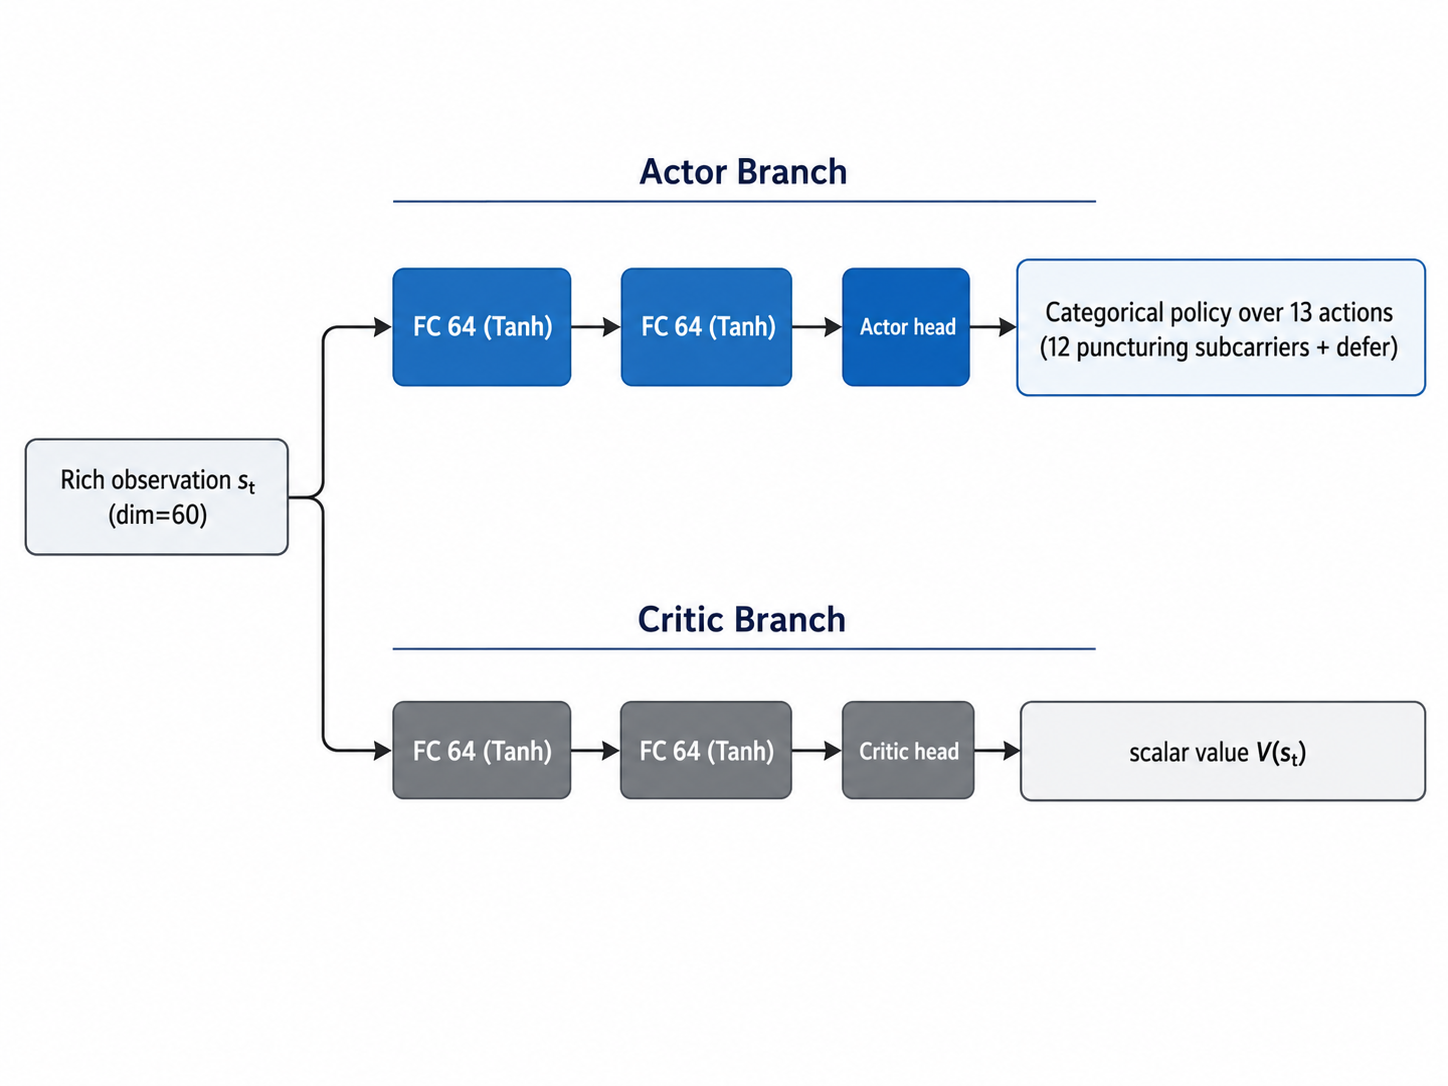
\includegraphics[width=0.9\textwidth]{PPO Actor-Critic网络结构.png}
\caption{PPO Actor-Critic 网络结构}
\label{fig:ppo_actor_critic}
\end{figure}

在深度强化学习中，Actor（策略）与 Critic（价值）网络的结构设计对训练稳定性至关重要。原基线文献\cite{saggese2021}采用了具有 128-64-32 三层全连接（ReLU 激活）的较深网络；而在本研究的实际工程实现中，为避免过拟合并提高梯度更新的稳定性，本文基于 Stable-Baselines3 (SB3) 框架，采用了标准 \texttt{MlpPolicy} 架构。

动作空间采用严格离散的 \texttt{Discrete(13)}，策略网络和价值网络在训练时关注的目标不同，如果共用后续隐藏层，容易让策略梯度和价值预测梯度互相牵制，因此模型在完成特征提取后，把网络拆成 Actor 与 Critic 两个分支的多层感知机结构：

输入端接收 60 维 \texttt{rich} 状态向量（与本文训练配置对应），展平后送到两个独立分支中；Actor 分支有两层全连接层，每层 64 个神经元，激活函数使用 Tanh，Critic 分支也使用两层 64 维全连接层，并保持相同激活函数；这里选用 Tanh 而不是 ReLU，是为了让特征取值变化更平稳，减少离散动作 logits 被推得过于极端的情况；Actor 输出头使用离散 Categorical 策略，生成 13 维 logits，再经过 Softmax 转换成各子载波和 Defer 动作的选择概率，Critic 输出头给出一个标量状态价值，用来估计当前状态后续可能得到的折扣回报。

\subsection{鲁棒性评估方案与启发式基线}\label{342-ux9c81ux68d2ux6027ux8bc4ux4f30ux65b9ux6848ux4e0eux542fux53d1ux5f0fux57faux7ebf}

为充分验证所提算法（尤其是 \texttt{RANSlicingEnvVar} 环境中频域打孔负载均衡惩罚的效用），本研究设计了严格的分布外（Out-of-Distribution, OOD）泛化测试协议。

\begin{enumerate}
\def\labelenumi{\arabic{enumi}.}
\item
  高负载泛化测试（Robustness Test）：在标准训练阶段，URLLC 泊松到达率固定为 \(\lambda=0.5\)。在评估阶段，引入越界到达率梯度测试序列 \(\Lambda_{\text{test}} = \{0.2, 0.4, 0.6, 0.8, 1.0, 1.2, 1.5\}\)，并在每个 \(\lambda\) 下独立运行 \(E=50\) 个 episode（每个 episode 长度 \(T=140\)）。该测试旨在比较 PPO 与 VarPPO 在流量分布迁移下的 URLLC 违约率和 eMBB 中断率变化，而不是假设任一策略在极端负载下仍可保持零违约。
\item
  对比基线算法：主实验保留 \texttt{fixed\_static} 与 \texttt{fixed\_rr} 两个非学习型基线。\texttt{fixed\_static} 总是输出动作 \(a_t=0\)，用于展示最朴素静态抢占策略的表现；\texttt{fixed\_rr} 不依赖状态观测，其在时步 \(t\) 的确定性动作输出为 \(a_t^{\mathrm{RR}} = t \bmod F = t \bmod 12\)，用于提供较强的轮询启发式参考。
\end{enumerate}

主要实验参数设定汇总：

\begin{table}[htbp]
\centering
\small
\caption{主要实验参数设定汇总}
\label{tab:experiment_hyperparameters}
\renewcommand{\arraystretch}{1.2}
\begin{tabularx}{\textwidth}{@{}>{\raggedright\arraybackslash}p{0.26\textwidth}>{\raggedright\arraybackslash}p{0.14\textwidth}>{\raggedright\arraybackslash}X@{}}
\toprule
超参数/实验参数 & 符号 & 设定取值与工程逻辑 \\
\midrule
PPO 学习率 & \(\eta\) & \(3\times 10^{-4}\)（与训练实验设定一致） \\
PPO 折扣因子 & \(\gamma\) & 0.99（Stable-Baselines3 PPO 默认值） \\
裁剪系数 & \(\epsilon\) & 0.2（Stable-Baselines3 PPO 默认值） \\
熵奖励系数 & \(c_2\) & 0.0（代码未额外设置熵奖励） \\
每轮采样步数 & \(n_{\mathrm{steps}}\) & 1400（即 10 个 episode 的采样长度） \\
批量大小 & -- & 140（即 1 个 episode 的步数） \\
训练总步数 & -- & 200000 \\
VarPPO 均衡惩罚总系数 & \(\alpha\) & 1.0（训练与鲁棒性测试实际取值） \\
VarPPO 分项权重 & \(w_i\) & load/margin/thr 均为 0.5，roll 为 0.2（归一化后经验标定，未进行完备网格搜索） \\
测试回合数 & \(E_{\mathrm{eval}}\) & 50（鲁棒性泛化测试）/ 100（常规测试） \\
到达率测试域 & \(\Lambda_{\text{test}}\) & \(\{0.2,0.4,0.6,0.8,1.0,1.2,1.5\}\)（覆盖轻载至极重载场景） \\
均衡惩罚动机 & 风险规避 & 通过频域打孔负载均衡吸收文献 \cite{alsenwi2021} 的风险规避思想 \\
\bottomrule
\end{tabularx}
\end{table}

\section{本章小结}\label{35-ux672cux7ae0ux5c0fux7ed3}


本章主要讨论 5G NR 空口中 eMBB 与 URLLC 业务同时存在时的资源调度问题，并围绕这个问题完成了仿真环境、队列变化模型、MDP 要素定义和 PPO 工程实现等内容，形成了一条从系统建模到算法验证的完整设计流程\cite{saggese2021}。

第一点，系统模型基于 Gymnasium 框架搭建，仿真里的时间结构也尽量向 5G NR 帧结构靠近；时域上采用 Slot（时隙）和 Mini-slot（微时隙）两级划分，相干时间取 10 ms，每个 1 ms Slot 再分成 14 个 Mini-slot，因此单个回合一共有 \(T = 140\) 个调度时步；频域上把系统带宽划成 \(F = 12\) 个互相正交的物理资源块，从而形成完整的时频资源网格；物理层部分没有继续做复杂的信道编码仿真，而是用整数打孔容忍度 \(\tau_f \sim \text{Uniform}\{1,2,3,4\}\) 表示 eMBB 码字能够承受的抢占程度，这样既能保留不同码字之间的风险差别，也能给后面加入风险规避机制留下更细的容忍度刻度。

第二点，URLLC 数据包的到达过程用泊松过程描述，考虑到 3GPP 对 1 ms 端到端时延的限制，每个新包的初始剩余时限从基线文献里的 \(D=7\) 收紧到 \(D=3\) 个 Mini-slot（约 0.21 ms），这样能给空口传输和硬件处理留出一定余量，同时也让调度问题更贴近超低时延业务会遇到的压力场景；在这个基础上，队列状态更新方程从新包到达、服务离队、时限递减和超时清理四个角度描述队列中数据包的变化关系，后面计算奖励信号时也有了对应依据\cite{alsenwi2021}。

第三点，MDP 建模采用 Perfect-CSI 辅助的 tolerance-aware 观测方式，把 eMBB 码字可靠性裕度 \(C_w\) 当作理想可观测的 oracle-assisted 上界变量，用它说明在完美信道可观测条件下，算法大概能达到怎样的性能上限；动作空间采用离散分类策略，这和 5G 物理层打孔机制中“选中某个资源块或暂缓”的互斥特点比较一致，也能减少连续动作取整带来的梯度问题；奖励函数分成两类，一类是基线稠密奖励，用持续步进惩罚代替只在终止时给出的稀疏惩罚，另一类是 VarPPO 奖励，在基线奖励上加入频域打孔负载均衡项，通过打孔计数方差和剩余裕度方差减少 eMBB 风险向少数子载波集中，同时用码字吞吐状态方差和滚动吞吐方差对短期稳定性再做补充约束\cite{alsenwi2021}。

算法实现使用 Stable-Baselines3 框架，并采用双分支 Actor-Critic 网络结构，Actor 和 Critic 都保留两层 64 维全连接隐藏层，激活函数设为 Tanh，这种结构能让离散动作 logits 的变化更平滑一些；评估方案采用分布外（OOD）泛化测试协议，主性能图比较四类调度策略，鲁棒性图只比较 PPO 与 VarPPO，并在到达率序列 \(\Lambda_{\text{test}} = \{0.2, 0.4, \ldots, 1.5\}\) 上观察频域打孔负载均衡奖励在流量分布变化时产生的影响\cite{saggese2021}。

经过上述建模与实现，第三章形成了统一、可复现的系统模型和算法评估框架，后续章节可以在同一基准下开展对比实验和机理分析，也能为 6G 超低时延网络切片调度相关仿真提供参考。


\chapter{仿真实验与结果分析}\label{ux56dbux4effux771fux5b9eux9a8cux4e0eux7ed3ux679cux5206ux6790}

本章主要介绍基于深度强化学习的 5G RAN（无线接入网）切片资源分配算法的仿真实验过程与综合结果，一方面给出自建 Gymnasium 仿真环境的具体配置，并通过表格列出离散化系统模型参数与强化学习智能体的训练超参数；另一方面从训练收敛性、综合评级分数、URLLC 违约率、eMBB 中断率以及负载均衡方差等维度，对静态抢占、确定性轮询、基线 PPO（Vanilla PPO）和 VarPPO 进行对比。PPO 与 VarPPO 的训练奖励不具备直接可比性，主结果以所有方法共享的综合评级分数 \(S_{\text{eval}}\) 为公平比较口径；在跨梯度 URLLC 突发流量到达率（\(\lambda \in [0.2, 1.5]\)）测试中，本章仅比较 PPO 与 VarPPO 在分布外（Out-of-Distribution, OOD）负载迁移下的鲁棒性表现。

\section{仿真环境设置与网络参数配置}\label{41-ux4effux771fux73afux5883ux8bbeux7f6eux4e0eux7f51ux7edcux53c2ux6570ux914dux7f6e}

为了客观、可重复地评估深度强化学习算法在混合切片场景下的调度性能，本研究基于 Python 语言与 Gymnasium 强化学习框架，构建了定制化的单小区 RAN 切片仿真环境，并分别实现了基础违约/中断惩罚环境与频域负载均衡奖励环境。

如第三章所述，该环境没有展开底层链路级（Link-level）复杂仿真，而是对 5G 物理层（PHY）的信道解码与媒体接入控制层（MAC）的时频资源网格调度过程进行离散化与降维抽象，以保证强化学习状态空间与动作空间在计算上的可解性。

\subsection{仿真场景与核心业务参数设定}\label{411-ux4effux771fux573aux666fux4e0eux6838ux5fc3ux4e1aux52a1ux53c2ux6570ux8bbeux5b9a}

本章仿真使用的基础参数沿用第三章中的系统模型，具体见表~\ref{tab:sim_core_params}。

在流量模型和业务限制方面，主要有两个部分：

\begin{itemize}

\item
  eMBB 业务：这里把 eMBB 业务看成满缓冲区（Full-buffer）状态下的连续数据流，它的数据队列一直有数据，不会出现空队列，系统分配给它的子载波资源基本都能被填满；物理层中较复杂的信道衰落和解码过程，在仿真中用每个子载波上的随机打孔容忍度来代替，即 \(\tau_f \sim \text{Uniform}\{1,2,3,4\}\)。
\item
  URLLC 业务：这里用泊松过程（Poisson Process）描述 URLLC 的突发到达，在微时隙 \(t\) 内的到达量为 \(A(t) \sim \text{Poisson}(\lambda)\)；考虑到 URLLC 对时延很敏感，队列最大等待时间（Deadline）设为 \(D=3\) 个微时隙，一旦超过这个时间就记为违约丢包。
\end{itemize}

\begin{longtable}[]{@{}>{\raggedright\arraybackslash}p{0.30\textwidth}>{\raggedright\arraybackslash}p{0.20\textwidth}>{\raggedright\arraybackslash}p{0.42\textwidth}@{}}
\caption{RAN 切片仿真环境核心参数}\label{tab:sim_core_params}\\
\toprule\noalign{}
参数名称 & 取值 & 物理意义 \\
\midrule\noalign{}
\endhead
\bottomrule\noalign{}
\endlastfoot
频域资源总量（Total Subcarriers） & \(F = 12\) & 离散抢占动作维度 \\
调度回合长度（Episode Length） & \(T = 140\) 步 & 每回合总微时隙数（\(10 \times 14\)） \\
eMBB 打孔容忍度（Tolerance） & \(\tau_f \in \{1,2,3,4\}\) & 码字中断前可承受打孔上限 \\
URLLC 时延约束（SLA Deadline） & \(D = 3\) 步 & 超过 3 个微时隙即计违约 \\
URLLC 基础到达率（Base \(\lambda\)） & \(0.5\) 包/步 & 训练与常规评估的泊松均值 \\
URLLC 泛化测试域（OOD \(\lambda\)） & \([0.2, \dots, 1.5]\) & 轻载到重载的压力测试区间 \\
资源调度粒度（Granularity） & 1 包 / 微时隙 & 每步最多服务 1 个 URLLC 包 \\
动作空间（Action Space） & \(\mathrm{Discrete}(F+1)\) & 12 个子载波抢占动作 + 1 个 Defer 动作 \\
PPO/VarPPO 观测模式 & \texttt{rich} & 默认维度 60，包含 Perfect-CSI 理想可靠性裕度与历史反馈 \\
\end{longtable}

\subsection{强化学习智能体与超参数配置}\label{412-ux5f3aux5316ux5b66ux4e60ux667aux80fdux4f53ux4e0eux8d85ux53c2ux6570ux914dux7f6e}

为了全面评估所提算法在高动态网络中的性能，本章设计了四组对比调度策略进行基准测试：

\begin{enumerate}
\def\labelenumi{\arabic{enumi}.}

\item
  \texttt{fixed\_static}（静态抢占基线）：最朴素的非学习型策略，始终选择 0 号子载波进行抢占。该策略用于反映不感知队列、时限和可靠性裕度时的静态基线表现。
\item
  \texttt{fixed\_rr}（确定性轮询算法）：传统的无模型、非学习型启发式基线，该策略不读取系统状态，只按照 \(a_t = t \bmod 12\) 做循环映射，因此能作为较有代表性的轮询参考，但它不能覆盖所有可能的基线方案。
\item
  基线 PPO（Vanilla PPO）：采用经典 Actor-Critic 架构的智能体，观测信息包括队列、时延、时隙位置和可靠性裕度等维度；奖励函数 \(R_{\text{base}}\) 使用稠密步进惩罚，只把 URLLC 超时违约（权重 1.0）和 eMBB 首次传输中断（权重 0.5）按线性方式合成。
\item
  VarPPO（频域负载均衡 PPO）：运行在均衡奖励环境中，观测模式为 \texttt{rich}，均衡惩罚总系数设为 \(\alpha=1.0\)，观测空间与 PPO 保持一致，但训练奖励中额外加入打孔计数方差、剩余裕度方差、码字吞吐状态方差和滚动吞吐方差惩罚；前两项主要约束频域打孔负载是否均衡，后两项用来辅助描述短期服务稳定性。
\end{enumerate}

深度强化学习的性能会受到超参数设定影响，本文的超参数设置基本对齐 Stable-Baselines3 框架中 PPO 的标准实现；除表~\ref{tab:ppo_hparams} 已列出的项目外，其余参数都沿用框架默认值，具体训练超参数如下所示。

\begin{table}[htbp]
\centering
\caption{PPO 强化学习算法超参数配置}
\label{tab:ppo_hparams}
\begin{tabular}{@{}>{\raggedright\arraybackslash}p{0.30\textwidth}>{\raggedright\arraybackslash}p{0.20\textwidth}>{\raggedright\arraybackslash}p{0.42\textwidth}@{}}
\toprule
超参数 & 设定值 & 说明 \\
\midrule
策略网络类型 & 多层感知机策略 & Actor 与 Critic 均采用前馈神经网络结构 \\
网络结构 & \([64,64]\) & Actor 与 Critic 均采用两层 64 维隐藏层，激活函数为 Tanh \\
学习率 \(\eta\) & \(3 \times 10^{-4}\) & PPO 策略网络与价值网络采用相同学习率 \\
折扣因子 \(\gamma\) & 0.99 & 采用 Stable-Baselines3 PPO 默认值 \\
GAE 参数 \(\lambda_{\text{GAE}}\) & 0.95 & 采用 Stable-Baselines3 PPO 默认值 \\
裁剪阈值 \(\epsilon\) & 0.2 & 采用 Stable-Baselines3 PPO 默认值 \\
价值损失系数 \(c_1\) & 0.5 & 采用 Stable-Baselines3 PPO 默认值 \\
熵系数 \(c_2\) & 0.0 & 未额外引入熵奖励 \\
每轮采样步数 \(n_{\text{steps}}\) & 1400 & 对应 10 个 episode 的交互样本 \\
批量大小（Batch Size） & 140 & 对应 1 个 episode 的交互样本 \\
训练轮数 \(n_{\text{epochs}}\) & 10 & 每次 rollout 后的 PPO 优化轮数 \\
训练总步数 & 200000 & PPO 与 VarPPO 均采用相同步数 \\
随机种子 & 42 & PPO 与 VarPPO 均采用相同 seed \\
VarPPO 均衡惩罚总系数 \(\alpha\) & 1.0 & 频域负载均衡奖励的总权重 \\
\bottomrule
\end{tabular}
\end{table}

\section{深度强化学习算法训练收敛性与微观策略演化分析}\label{42-ux6df1ux5ea6ux5f3aux5316ux5b66ux4e60ux7b97ux6cd5ux8badux7ec3ux6536ux655bux6027ux4e0eux5faeux89c2ux7b56ux7565ux6f14ux5316ux5206ux6790}

深度强化学习主要靠试错（Trial-and-Error）来更新策略，智能体会多次和底层 MAC 层环境交互，所以训练过程能不能平稳收敛，可以比较直接地看出奖励函数设置是否合适；本文在基础训练场景（\(\lambda=0.5\)）下，让基线 PPO 和 VarPPO 采用相同步长进行在线训练，再通过累积奖励曲线观察神经网络在不同训练阶段处理多目标优化时的策略变化。

\begin{figure}[H]
\centering

\includegraphics[width=0.9\textwidth]{training_curves.png}
\caption{PPO 与频域负载均衡 PPO 的训练收敛对比曲线}
\label{fig:training_curves}
\end{figure}

图~\ref{fig:training_curves} 给出了两种 PPO 智能体在各自训练目标下的学习过程，两条曲线随着训练推进整体上升，说明标准 PPO 和 VarPPO 都能从多维状态观测中学到比初始随机策略更稳定的抢占决策；不过 VarPPO 多加入了方差惩罚项，即时奖励的尺度和标准 PPO 不一样，因此不能只用累计奖励的数值大小来直接比较二者好坏。

这条曲线主要用来说明一点：状态空间加入多维观测后，特别是加入 \(C_w\) 可靠性裕度后，智能体仍然能完成稳定训练，并且能得到可用的调度策略；另一方面，VarPPO 虽然面对的是更偏向风险控制的训练目标，但曲线中仍有明显学习趋势，这说明频域打孔负载均衡惩罚没有影响 PPO 的基本优化过程；后面真正做公平比较时，仍要回到所有方法共用的综合评级分数 \(S_{\text{eval}}\)、URLLC violation rate、eMBB outage rate 以及方差类指标。

\section{基础场景下的系统综合性能对比}\label{43-ux57faux7840ux573aux666fux4e0bux7684ux7cfbux7edfux7efcux5408ux6027ux80fdux5bf9ux6bd4}

为量化评估训练收敛后各智能体的调度能力，本节在 \(\lambda=0.5\) 的验证环境中进行独立测试回合。条形图（图~\ref{fig:performance_bar}）比较静态抢占、确定性轮询、基线 PPO 与 VarPPO 四种方法，并采用所有方法共享的综合评级分数 \(S_{\text{eval}}\) 作为主指标。其定义与式~\eqref{eq:s_eval} 一致，其中 \(N_{\text{URLLC}}^{\text{viol}}\) 和 \(N_{\text{eMBB}}^{\text{out}}\) 分别表示单个测试回合内的 URLLC 时延违约次数和 eMBB 码字中断次数。该图同时给出 URLLC violation rate、eMBB outage rate、\(\mathrm{Var}(\mathbf{b})\)、\(\mathrm{Var}(\tilde{\mathbf{p}})\) 和 \(\mathrm{Var}(\tilde{\mathbf{g}})\) 等辅助指标。

\begin{figure}[H]
\centering
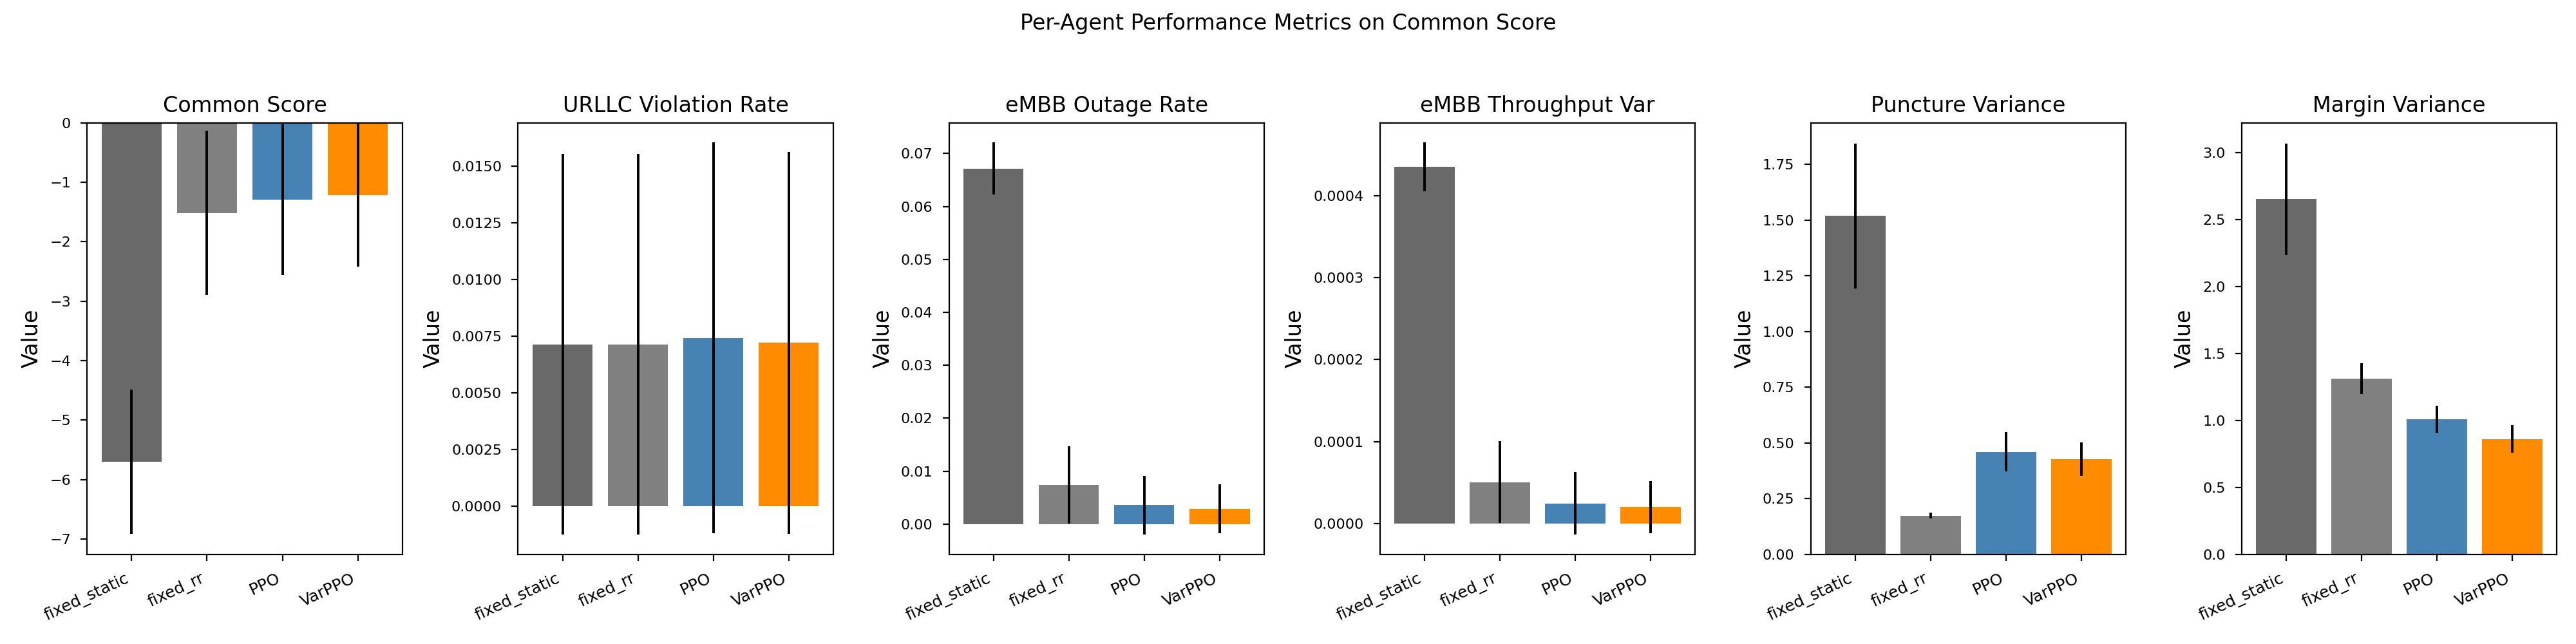
\includegraphics[width=0.98\textwidth]{performance_bar.png}
\caption{基础场景下不同调度策略的关键性能指标对比}
\label{fig:performance_bar}
\end{figure}

图~\ref{fig:performance_bar} 中的综合评级分数越高越好，因为它直接对应 URLLC 违约与 eMBB 中断的共同惩罚。其余错误率与方差类指标则越低越好。与训练曲线不同，\(S_{\text{eval}}\) 对 PPO 与 VarPPO 使用同一评价函数，因此可作为二者最终策略质量的公平比较依据。

基于模型收敛后的策略权重，本文在独立生成的 100 个验证回合中进行了性能评估。图~\ref{fig:performance_bar} 六个子图对应的原始统计值如表~\ref{tab:performance_bar_data} 所示。其中，URLLC 违约率与 eMBB 中断率均由每回合总次数除以 episode 长度 \(T=140\) 得到；表中误差项为 100 个测试回合上的标准差。

\begin{table}[H]
\centering
\small
\caption{基础场景下性能柱状图对应的原始评估数据}
\label{tab:performance_bar_data}
\resizebox{\textwidth}{!}{%
\begin{tabular}{lcccccc}
\hline
方法 & \(S_{\text{eval}}\) & URLLC Violation Rate & eMBB Outage Rate & \(\mathrm{Var}(\mathbf{b})\) & \(\mathrm{Var}(\tilde{\mathbf{p}})\) & \(\mathrm{Var}(\tilde{\mathbf{g}})\) \\
\hline
\texttt{fixed\_static} & \(-5.700\pm1.212\) & \(0.0071\pm0.0084\) & \(0.0671\pm0.0050\) & \(4.35{\times}10^{-4}\pm2.99{\times}10^{-5}\) & \(1.52\pm0.326\) & \(2.65\pm0.418\) \\
\texttt{fixed\_rr} & \(-1.515\pm1.379\) & \(0.0071\pm0.0084\) & \(0.0074\pm0.0073\) & \(5.03{\times}10^{-5}\pm4.97{\times}10^{-5}\) & \(0.174\pm0.0138\) & \(1.31\pm0.116\) \\
\texttt{PPO} & \(-1.290\pm1.269\) & \(0.0074\pm0.0086\) & \(0.0036\pm0.0056\) & \(2.45{\times}10^{-5}\pm3.81{\times}10^{-5}\) & \(0.459\pm0.0880\) & \(1.01\pm0.102\) \\
\texttt{VarPPO} & \(-1.215\pm1.209\) & \(0.0072\pm0.0084\) & \(0.0029\pm0.0046\) & \(2.01{\times}10^{-5}\pm3.18{\times}10^{-5}\) & \(0.426\pm0.0752\) & \(0.861\pm0.104\) \\
\hline
\end{tabular}
}
\vspace{0.5em}
\begin{minipage}{0.96\textwidth}
\footnotesize
注：\(\mathbf{b}=1-\mathbf{O}\) 表示归一化 eMBB 码字服务状态，\(\tilde{\mathbf{p}}\) 表示归一化打孔计数向量，\(\tilde{\mathbf{g}}\) 表示归一化剩余可靠性裕度向量；这些方差都是按子载波维度统计得到的无量纲指标，不能把它们理解成以 Mbps 或 bit/s 为单位的物理吞吐量方差。
\end{minipage}
\end{table}

从综合评级分数看，\texttt{fixed\_static} 的平均得分为 \(-5.700\)，明显低于另外三种方法，这说明 URLLC 到达后如果一直抢占同一个子载波，就会很快用掉该频段上 eMBB 码字的容忍度，主要惩罚也会集中表现为 eMBB 中断；相比之下，\texttt{fixed\_rr} 通过轮询把打孔影响分到不同子载波上，使 \(S_{\text{eval}}\) 提升到 \(-1.515\)，PPO 又提升到 \(-1.290\)，这说明智能体在用到队列、时隙位置和理想可靠性裕度等多维观测后，能学到比固定轮询更会看状态的抢占策略；VarPPO 的 \(S_{\text{eval}}\) 达到 \(-1.215\)，比 PPO 高 \(0.075\)，相当于公共惩罚幅度约降低 \(5.8\%\)，比 \texttt{fixed\_rr} 高 \(0.300\)，相当于公共惩罚幅度约降低 \(19.8\%\)，从实验结果看，频域负载均衡机制在保持 URLLC 时延达标率的同时，也能对 eMBB 中断控制和稳定性指标带来比较温和的改善。

从 URLLC violation rate 看，四种方法都处在 \(0.0071\sim0.0074\) 这个比较窄的区间内，换到每 140 个 mini-slot 的 episode 中，大约只会有 1 次 URLLC 时延违约；\texttt{fixed\_static} 和 \texttt{fixed\_rr} 的平均违约次数都是 \(1.000\) 次/回合，PPO 为 \(1.040\) 次/回合，VarPPO 为 \(1.010\) 次/回合，这说明在基础到达率 \(\lambda=0.5\) 下，各策略在 URLLC 侧的服务能力差别不大，学习型方法的优势不是靠牺牲或明显改变 URLLC 服务率换来的；VarPPO 的 URLLC violation rate 比 PPO 稍低，但差值仍然小于标准差范围，所以更适合把它看成统计波动下的基本持平，而不是 URLLC 时延保障能力有了明显提升。

从 eMBB outage rate 看，不同策略之间的差别更明显，\texttt{fixed\_static} 的 eMBB outage rate 为 \(0.0671\)，也就是平均每回合会有 \(9.400\) 次 eMBB 中断；\texttt{fixed\_rr} 降到 \(0.0074\)，平均 \(1.030\) 次/回合，说明简单的均匀轮询已经能明显减少对同一个 eMBB 码字的持续挤压；PPO 继续把这个指标降到 \(0.0036\)，平均 \(0.500\) 次/回合，比 \texttt{fixed\_rr} 约少 \(51.5\%\)，比 \texttt{fixed\_static} 约少 \(94.7\%\)；VarPPO 的 eMBB outage rate 最低，为 \(0.0029\)，平均 \(0.410\) 次/回合，比 PPO 又少约 \(18.0\%\)，因此图中综合评级分数变好，主要来自 eMBB 中断控制的改善，而不是 URLLC violation 出现了很大变化。

归一化 eMBB 吞吐状态方差和中断率的变化方向基本一致，静态抢占策略的方差达到 \(4.35\times10^{-4}\)，比其他几种方法高出不少，这说明一直在同一个频段上打孔，会让短时间内的服务状态起伏更大；确定性轮询把该值降到 \(5.03\times10^{-5}\)，PPO 又降到 \(2.45\times10^{-5}\)，VarPPO 最低，为 \(2.01\times10^{-5}\)，比 PPO 低了约 \(18.0\%\)，比确定性轮询低了约 \(60.0\%\)；这里的方差来自归一化后的码字服务状态统计，数值本来就会比较小，这是归一化建模后会出现的正常量级，不能把它看成真实物理层吞吐量中以 Mbps 为单位的方差；从这组结果可以看出，频域负载均衡在保持 URLLC 时延达标情况基本不变的同时，也能让 eMBB 的服务稳定性有一定改善。

puncture-count variance 不能只看数值大小，还要放到各策略的动作方式里理解，\texttt{fixed\_rr} 的打孔计数方差最低，只有 \(0.174\)，主要原因是轮询策略会按子载波编号一个接一个地循环，它天然会把打孔次数摊平，但这不代表它真的读懂了队列状态或者可靠性状态；PPO 和 VarPPO 的打孔方差分别为 \(0.459\) 和 \(0.426\)，这两个数都高于 \texttt{fixed\_rr}，但比 \texttt{fixed\_static} 的 \(1.52\) 低很多，说明学习型策略并不是只想做到“每个子载波被打孔次数完全一样”，而是会在 URLLC deadline、当前 slot/mini-slot 位置、eMBB 可靠性裕度之间取一个折中；VarPPO 比 PPO 又低了约 \(7.2\%\)，说明加入负载均衡惩罚以后，策略偏好确实有变化，不过这个变化比较平缓，并没有把策略硬改成简单轮询。

从 remaining-margin variance 来看，VarPPO 的设计意图会更明显一些，这个指标反映不同子载波剩余可靠性裕度 \(C_w-p_f(t)\) 拉开的程度；\texttt{fixed\_static} 的 margin variance 达到 \(2.65\)，说明持续打孔会让少数子载波的裕度很快下降，其他子载波却还有较多空余，可靠性风险就集中到了少数位置；\texttt{fixed\_rr} 把该值降到 \(1.31\)，PPO 继续降到 \(1.01\)，VarPPO 最低，为 \(0.861\)，比 PPO 低约 \(14.8\%\)，比 \texttt{fixed\_rr} 低约 \(34.3\%\)，这和 VarPPO 在奖励里直接惩罚剩余裕度方差的设计比较一致，说明它不只是减少总的中断次数，也会在更细的子载波层面上，把各个 eMBB 码字的可靠性余量保护得更均衡。

把六个指标放在一起看，\texttt{fixed\_static} 更像是一个反面参照，它说明“总在同一个位置打孔”会明显破坏 eMBB；\texttt{fixed\_rr} 是一个效果不错的负载均衡启发式方法，特别是在 puncture-count variance 上最好，但它没有用到系统状态，所以在 eMBB outage、归一化吞吐状态方差、剩余裕度方差这些指标上，还是不如学习型策略；PPO 用到了多维状态观测以后，对 eMBB 中断有了更好的控制；VarPPO 又在 PPO 的基础上，把综合评级分数、eMBB outage rate、normalized eMBB throughput variance 和 remaining-margin variance 做了进一步改善，只是提升幅度不是特别大；因此，本文对 VarPPO 的贡献做一个比较稳妥的说明，即它在不明显影响 URLLC 时延指标的前提下，通过频域打孔负载均衡改善了 eMBB 侧可靠性风险的分布，而不是说它在每一个单项指标上都一定强于启发式方法。

\section{频域打孔负载均衡与通信稳定性机理}\label{44-embbux541eux5410ux91cfux65b9ux5deeux4e0eux6df1ux5c42ux901aux4fe1ux7a33ux5b9aux6027ux673aux7406}

在无线资源调度中，不仅要评估宏观维度的误包率，也需要观察打孔压力是否被集中施加到少数子载波。图~\ref{fig:variance_dist} 的箱线图（Boxplot）展示的是每个 episode 内 per-subcarrier puncture-count variance 的分布，而不是训练 reward 或单步 eMBB 吞吐量本身。

\begin{figure}[H]
\centering
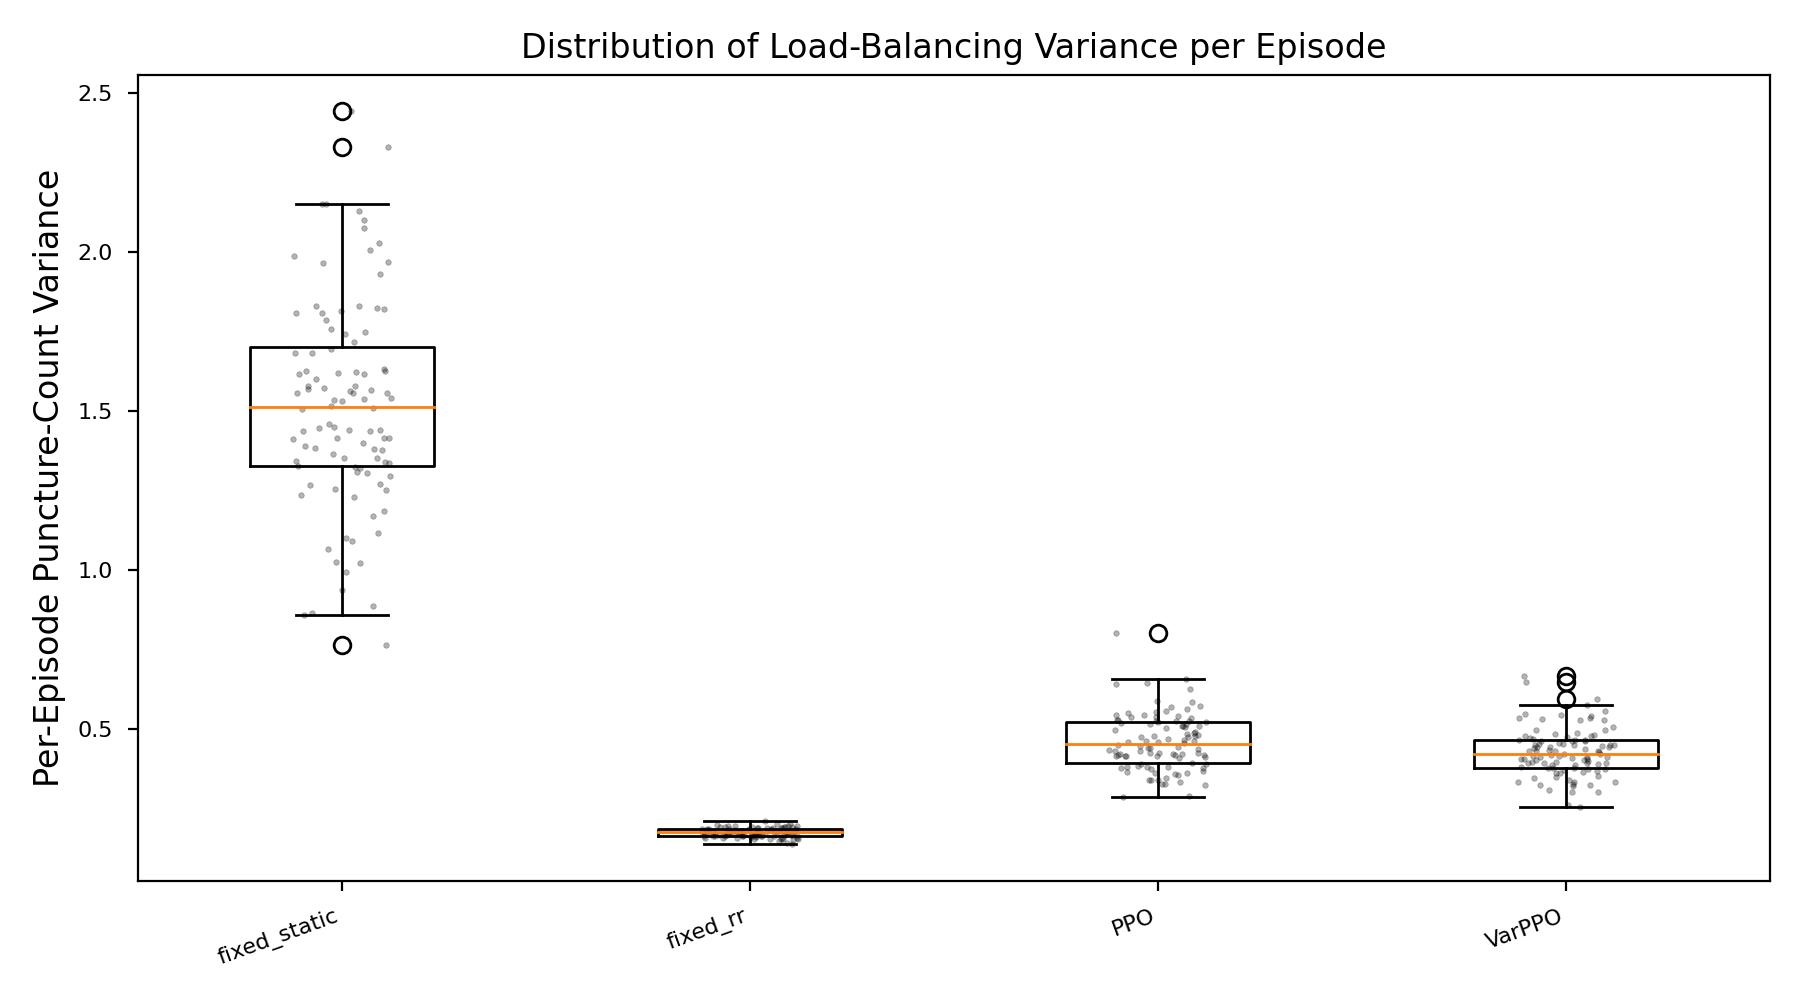
\includegraphics[width=0.9\textwidth]{variance_dist.png}
\caption{不同调度策略下打孔计数方差分布（按回合统计）}
\label{fig:variance_dist}
\end{figure}

打孔计数方差越低，说明 URLLC 对 eMBB 资源的频域抢占越均匀，单个码字或子载波被连续压榨到中断阈值附近的概率越小。为避免仅凭箱线图形状作定性判断，表~\ref{tab:puncture_variance_box_data} 列出了图~\ref{fig:variance_dist} 对应的原始分布统计量，包括均值、标准差、最小值、第一四分位数、中位数、第三四分位数和最大值。

\begin{table}[H]
\centering
\small
\caption{打孔计数方差箱线图对应的分布统计量}
\label{tab:puncture_variance_box_data}
\resizebox{\textwidth}{!}{%
\begin{tabular}{lccccccc}
\hline
方法 & Mean & Std & Min & Q1 & Median & Q3 & Max \\
\hline
\texttt{fixed\_static} & \(1.5179\) & \(0.3263\) & \(0.7633\) & \(1.3270\) & \(1.5120\) & \(1.7003\) & \(2.4428\) \\
\texttt{fixed\_rr} & \(0.1736\) & \(0.0138\) & \(0.1372\) & \(0.1633\) & \(0.1748\) & \(0.1842\) & \(0.2091\) \\
\texttt{PPO} & \(0.4589\) & \(0.0880\) & \(0.2860\) & \(0.3918\) & \(0.4521\) & \(0.5212\) & \(0.8006\) \\
\texttt{VarPPO} & \(0.4263\) & \(0.0752\) & \(0.2536\) & \(0.3771\) & \(0.4201\) & \(0.4641\) & \(0.6646\) \\
\hline
\end{tabular}
}
\end{table}

从整体分布看，静态策略的打孔方差均值为 \(1.5179\)，中位数为 \(1.5120\)，最大值达到 \(2.4428\)，显著高于其他三种策略。这与其动作机制完全一致：只要选择服务 URLLC，它总是打孔同一子载波，导致单个频段的打孔计数持续累积，而其他子载波几乎不承担抢占压力。因此，该策略的箱线图不仅位置最高，而且离散程度也最大，标准差达到 \(0.3263\)，说明不同 episode 中 URLLC 到达波动会进一步放大局部打孔压力的不稳定性。结合上一节的 eMBB outage rate 可知，这种高度集中的打孔分布会直接转化为更高的 eMBB 码字中断风险。

\texttt{fixed\_rr} 的打孔方差最低，均值仅为 \(0.1736\)，中位数为 \(0.1748\)，四分位区间约为 \([0.1633,0.1842]\)，标准差也只有 \(0.0138\)，这说明轮询策略在“打孔次数均匀性”这一单一维度上比较稳定，相比 \texttt{fixed\_static} 将平均打孔方差降低约 \(88.6\%\)；不过，这一结果主要由确定性的循环动作 \(a_t=t\bmod F\) 带来，并不是因为策略读入了 URLLC 队列、剩余 deadline 或 eMBB 码字裕度等状态信息，也就是说，\texttt{fixed\_rr} 的低方差更多体现了动作编号上的机械均匀，不一定代表它能把打孔放到当前最适合承受影响的码字上。

PPO 的打孔方差均值为 \(0.4589\)，高于 \texttt{fixed\_rr}，但相比 \texttt{fixed\_static} 仍降低约 \(69.8\%\)，其中位数为 \(0.4521\)，第一、第三四分位数分别为 \(0.3918\) 和 \(0.5212\)；这表明 PPO 学到的策略并不是简单复制轮询，而是会在队列状态、mini-slot 位置、打孔历史和可靠性裕度之间做权衡，当某些子载波还有更高剩余裕度，或者当前动作更有利于降低即时惩罚时，策略可能会有意识地偏向这些资源；因此，PPO 的打孔次数分布不如 \texttt{fixed\_rr} 均匀，但它在上一节中取得了更低的 eMBB outage rate 和更高的 \(S_{\text{eval}}\)，说明“适度不均匀”有时来自状态信息下的选择，并不等于调度失效。

VarPPO 的分布介于 PPO 与 \texttt{fixed\_rr} 之间，均值为 \(0.4263\)，中位数为 \(0.4201\)，相比 PPO 的均值降低约 \(7.1\%\)。更重要的是，VarPPO 的第三四分位数从 PPO 的 \(0.5212\) 降至 \(0.4641\)，最大值从 \(0.8006\) 降至 \(0.6646\)，四分位距也由 \(0.1294\) 缩小至 \(0.0870\)。这说明频域打孔负载均衡惩罚并未把策略强行拉成固定轮询，而是降低了高方差 episode 出现的概率，使打孔压力在训练策略内部得到更温和的分摊。该结果与 VarPPO 奖励函数中对 puncture-count variance 和 remaining-margin variance 的显式惩罚相一致，也解释了其在图~\ref{fig:performance_bar} 中对 eMBB outage rate、eMBB 吞吐方差和 remaining-margin variance 的同步改善。

因此，图~\ref{fig:variance_dist} 的核心含义不是简单地按打孔方差给四种方法排序，而是揭示不同策略的调度机理差异。\texttt{fixed\_rr} 在打孔计数方差上最低，但它缺少状态感知，无法根据 \(C_w\) 可靠性裕度和 URLLC 紧迫程度动态调整；PPO 能利用多维状态观测改善中断控制，但仍可能在部分 episode 中形成较高的打孔集中度；VarPPO 则在 PPO 的状态感知能力基础上，通过奖励塑造压低高方差尾部，使负载分摊更稳定。因而本文将图~\ref{fig:variance_dist} 作为策略机理分析，将图~\ref{fig:performance_bar} 中的 \(S_{\text{eval}}\) 作为主性能比较依据：低打孔方差是通信稳定性的一个重要侧面，但只有与 eMBB 中断率、剩余裕度分布和综合评级分数共同观察时，才能完整评价调度策略的优劣。

\section{算法时间复杂度与真实基站部署的计算开销分析}\label{45-ux7b97ux6cd5ux65f6ux95f4ux590dux6742ux5ea6ux4e0eux771fux5b9eux57faux7ad9ux90e8ux7f72ux7684ux8ba1ux7b97ux5f00ux9500ux5206ux6790}

面向 5G 以及后续 6G 场景的无线资源管理（RRM）算法，不能只看误包率、中断率这些网络性能指标，也要考虑算法本身会花多少计算时间；在真实 5G 基站（gNodeB）的分布式单元（DU）或者边缘云（MEC）里，MAC 层 URLLC 调度一般按微时隙（Mini-slot）来走，本实验环境中的单个微时隙约为 0.0714 ms，也就是把 10 ms 相干时间分成 10 个 Slot，每个 Slot 再包含 14 个微时隙；如果算法每次推理用时超过了目标控制周期，那么即使仿真性能比较好，在线部署也会遇到实际困难。

在空间复杂度方面，PPO 训练结束以后，线上主要用到 Actor 网络来做动作选择，本实验采用的是轻量级全连接多层感知机（MLP），它负责把输入状态空间 \(S\) 映射到输出动作空间 \(A\)，空间复杂度可以近似写成 \(\mathcal{O}(|S| \cdot H + H^2 + H \cdot |A|)\)，其中 \(|S|=60\)，\(|A|=13\)，\(H=64\) 表示隐藏层宽度；如果只算 Actor 前向推理需要保存的权重，参数量大约为 \(60\times64+64\times64+64\times13=8768\) 个权重，再加上一小部分偏置，用单精度浮点数（FP32）存储时也就是数十 KB；实际模型文件还会带有 Critic、优化器或者框架元数据，整体大概是数百 KB 量级，对仿真平台和边缘计算节点来说都不算重。

时间复杂度与推理时延（Inference Latency）： 算法的单次前向推断计算复杂度同样为 \(\mathcal{O}(|S|H + H^2 + H|A|)\)。对当前 \(60\)-\(64\)-\(64\)-\(13\) 的 Actor MLP 而言，若按一次乘法和一次加法约计为 2 次浮点运算，则单次前向传播的主要矩阵乘加开销约为 \(\mathrm{FLOPs}\approx 2(60\times64+64\times64+64\times13)=17536\)。即使加入偏置加法与 Tanh 激活函数，整体仍处于 \(2\times10^4\) FLOPs 左右的量级。在现代基站 BBU、边缘服务器或通用 x86/ARM 平台上，该规模的纯 MLP 推理通常可由 SIMD/AVX/NEON 等向量化指令高效执行，理论计算负担远低于复杂优化求解器。需要说明的是，本文没有对真实基站硬件或不同 CPU/GPU 平台进行专门推理时延测试；相关文献中 0.3\(\sim\)3.0 ms 的 PPO 调度器推理延迟可作为系统级参考，而上述 FLOPs 估算说明本文所用 Actor 网络本身并非主要计算瓶颈。

非学习型基线的复杂度也有不同工程含义，\texttt{fixed\_rr} 只需要维护当前轮询索引并执行 \(a_t=t\bmod F\)，调度开销为 \(\mathcal{O}(1)\)，因此适合作为毫秒级实时系统中的极低延迟基线；相比之下，如果每步都读取 \(F=12\) 个子载波的剩余裕度，再通过排序选择最优位置，启发式方法的典型复杂度会达到 \(\mathcal{O}(F\log F)\)，同时还可能带来状态读取和同步延迟；PPO/VarPPO 的优势并不在于比确定性轮询拥有更低的常数级复杂度，而在于用少量在线推理开销换取对高维状态的非线性映射能力，在当前仿真配置下，VarPPO 通过状态感知和奖励塑造取得了更低的 eMBB 中断率，也让剩余裕度分布更平滑；未来如果面向真实基站部署，还需要进一步测试模型在目标硬件上的端到端推理时延，并考虑通过 FPGA、DSP/NPU 或边缘 GPU 等加速方式降低控制环路时延。

\section{面向非稳态突发流量的分布外泛化（OOD）分析}\label{46-ux9762ux5411ux975eux7a33ux6001ux7a81ux53d1ux6d41ux91cfux7684ux5206ux5e03ux5916ux6cdbux5316oodux4e0e-bad-case-ux5faeux89c2ux5256ux6790}

在实际现网中，URLLC 的突发频率无法精确预知。为了验证频域打孔负载均衡奖励塑造在流量分布变化下的作用，本节对泊松到达率进行分布外（Out-of-Distribution, OOD）扫频测试，覆盖 \(\lambda \in \{0.2, 0.4, 0.6, 0.8, 1.0, 1.2, 1.5\}\)。当前鲁棒性图仅比较 PPO 与 VarPPO，用于直接观察二者在相同多维状态观测下、不同训练奖励对流量迁移的影响。

\begin{figure}[H]
\centering
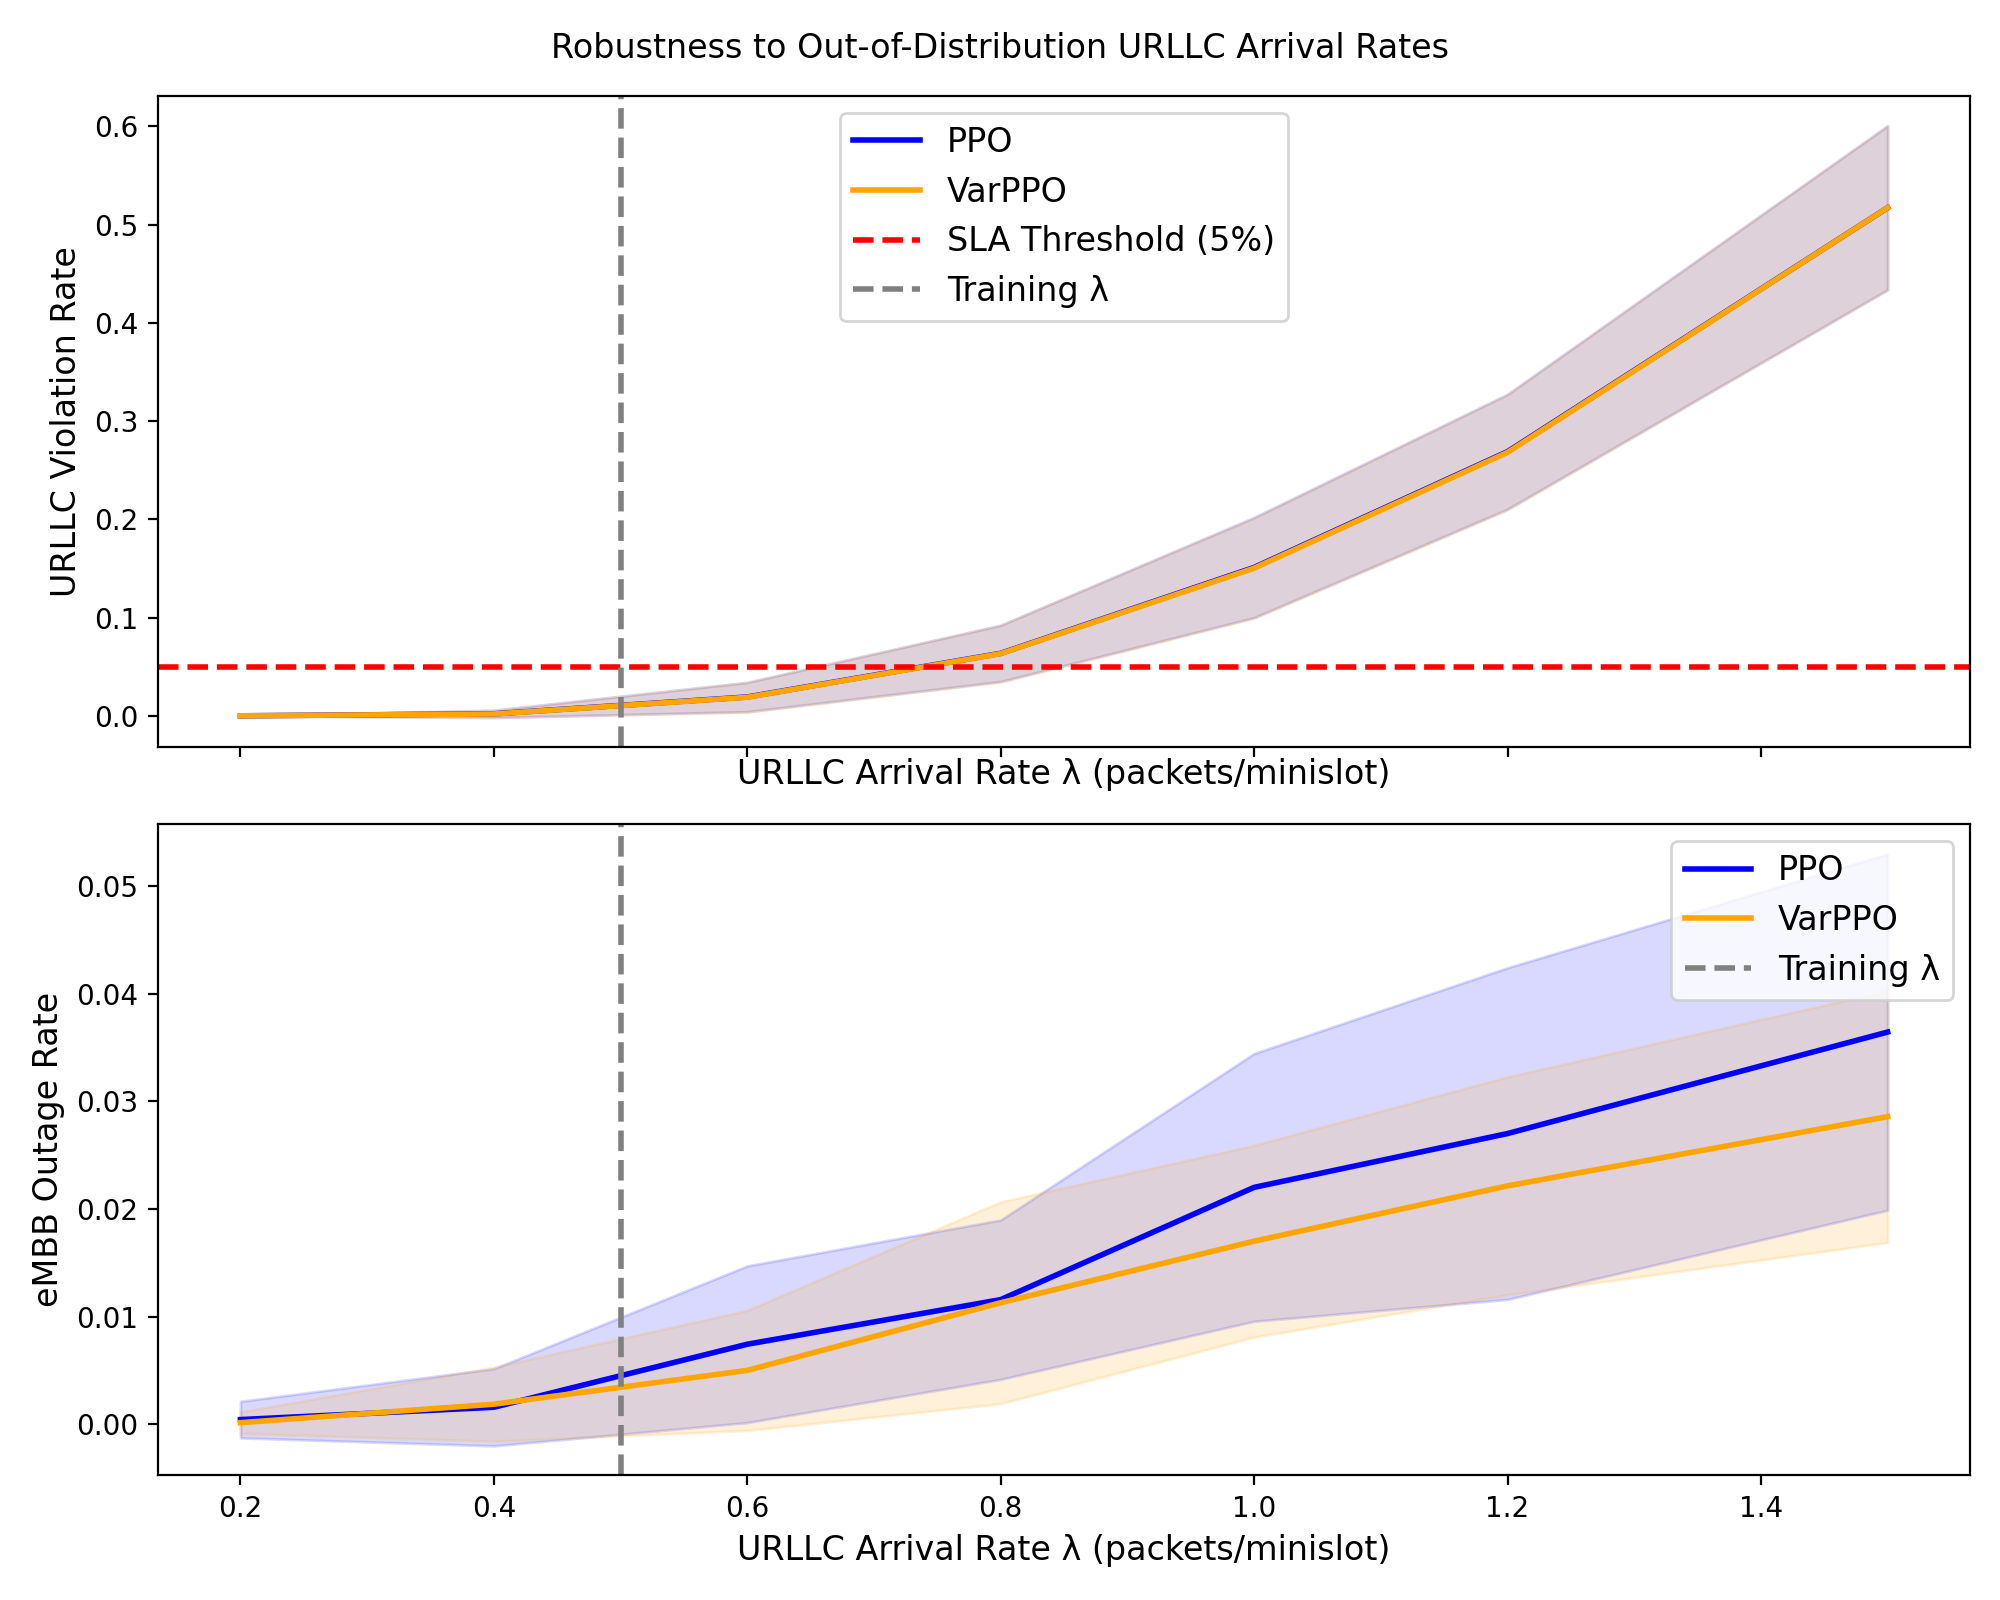
\includegraphics[width=0.9\textwidth]{robustness.png}
\caption{PPO 与 VarPPO 在分布外 URLLC 到达率下的鲁棒性对比}
\label{fig:robustness_ood}
\end{figure}

图~\ref{fig:robustness_ood} 包含 URLLC violation rate 与 eMBB outage rate 两个子图。二者都是错误率指标，因此曲线越低表示越好；图中的训练到达率 \(\lambda=0.5\) 用竖线标出，用于区分分布内与分布外测试区间。

当前结果显示，随着 \(\lambda\) 从 0.2 增加到 1.5，PPO 与 VarPPO 的 URLLC violation rate 基本接近；在 \(\lambda=1.5\) 时二者均约为 0.517。该现象可以从排队稳定性角度解释：本文环境中每个微时隙至多服务一个 URLLC 包，因此服务率上界为 \(\mu=1\) 包/微时隙。当到达率为 \(\lambda=1.5\) 时，系统负载率为 \(\rho=\lambda/\mu=1.5>1\)。这意味着即使不考虑有限 deadline，队列也已处于经典排队论意义上的不稳定区间，长期队列长度具有发散趋势；在 \(D=3\) 的硬时延约束下，这种容量不足会更快转化为时延违约。因此，极端负载下 URLLC violation rate 的急剧上升并不是某一调度策略的单独失效，而是到达过程超过服务能力后的物理容量边界。相比之下，VarPPO 在 eMBB outage rate 上更稳定，例如在 \(\lambda=1.0,1.2,1.5\) 时分别约为 0.0170、0.0221、0.0286，而 PPO 分别约为 0.0220、0.0270、0.0364。因此，本文将 VarPPO 的主要贡献解释为在流量迁移下改善 eMBB 中断控制，而不是声称其能够在极高负载下消除 URLLC 违约。

\section{本章小结}\label{47-ux672cux7ae0ux5c0fux7ed3}

本章基于接近 5G NR 标准的 MAC 层微时隙（Mini-slot）物理时序仿真环境，对静态抢占、确定性轮询、基线 PPO 和 VarPPO 四类方法做了对比，评价时同时看了 URLLC violation rate、eMBB outage rate、归一化吞吐状态方差、打孔计数方差、剩余裕度方差和综合评级分数 \(S_{\text{eval}}\)；其中，\(S_{\text{eval}}\) 采用统一口径计算，更适合拿来做不同方法之间的主比较，训练奖励曲线只用来说明 PPO 与 VarPPO 有没有学到有效策略，不能直接当成 VarPPO 一定优于 PPO 的证据。

从实验结果看，静态抢占因为长期压到同一频段，会让 eMBB 中断和短时服务波动都变得比较明显；确定性轮询能把打孔次数摊得更平均，但它没有读取队列、deadline 和可靠性裕度等状态，所以只能作为一个简单而稳定的启发式基线；PPO 用多维观测后，能够更好地控制 eMBB 中断，VarPPO 在此基础上加入负载均衡惩罚，使 eMBB outage rate、normalized eMBB throughput variance 和 remaining-margin variance 又有一定下降，不过提升幅度仍属于温和改善，不能扩大成所有指标全面领先。

本章还结合模型超参数、单次 Actor 前向传播约 \(1.75\times10^4\) FLOPs 的估算，以及不同基线策略的复杂度差异，讨论了轻量级 Actor 网络放到基站侧时的计算开销；在未见到达率（Out-of-Distribution, OOD）扫频测试中，本章只比较 PPO 和 VarPPO 的 URLLC violation rate 与 eMBB outage rate，并用 \(\rho>1\) 的排队不稳定条件说明极端负载下的性能边界，也就是说，当到达强度已经超过服务能力时，调度策略可以缓解 eMBB 侧风险，但不能从根本上消除 URLLC 违约。

\chapter{总结与展望}\label{ux4e94ux603bux7ed3ux4e0eux5c55ux671b}

\section{研究工作总结}\label{51-ux7814ux7a76ux5de5ux4f5cux603bux7ed3}

本文围绕``基于深度强化学习的 5G RAN 切片资源分配研究''这一主题展开，重点关注单小区下行链路中 URLLC 业务和 eMBB 业务同时存在时的资源竞争问题，其中 URLLC 对可靠性和时延要求很高，eMBB 则对带宽资源需求较大，两类业务放在同一套资源中调度时，会出现明显的动态冲突；针对这一问题，本文搭建了一个更贴近物理时序过程的强化学习仿真环境，并在此基础上设计了基于 PPO 的动态切片调度算法，同时选取固定规则调度方法（如 \texttt{fixed\_rr}）以及加入频域打孔负载均衡惩罚的改进策略（\texttt{VarPPO}）进行对比。结合仿真实验和理论分析，本文主要回应了研究目标中的三个问题：

一方面，针对``如何将 URLLC/eMBB 资源复用问题建模为 MDP''这个问题，本文把单小区下行切片里的抢占调度过程，整理成有限时域下的 tolerance-aware MDP；在这个 MDP 中，状态空间（State Space）主要记录 URLLC 数据包的泊松到达队列、还剩多少可容忍时延（Deadline）、当前时隙位置、eMBB 已经被打孔的次数、完美 CSI 假设下的理想可靠性裕度 \(C_w\)、剩余裕度，以及上一时步反馈等会随时间变化的信息，动作空间（Action Space）表示不同切片在具体时频资源块（RBs/FRs）上要不要抢占、抢占哪里，奖励函数（Reward Function）用来把 URLLC 时延违约带来的惩罚和 eMBB 服务质量损失放到同一个评价标准里；这样处理以后，抽象仿真环境能够表现出 MAC 层资源分配随时间变化时具有的马尔可夫特点，不过这些性能结果依然建立在理想信道可观测条件上，更适合当作理论上界来看。

另一方面，对于``如何设计兼顾 URLLC 时延约束、eMBB 中断控制和微观传输稳定性的奖励函数''这一问题，本文没有只依赖基础违约/中断惩罚，而是在奖励中加入了频域打孔负载均衡惩罚；这一设计主要围绕打孔计数方差和剩余裕度方差展开，用来限制不同子载波之间的打孔压力过度集中，同时把码字吞吐状态方差和滚动吞吐方差作为辅助项，用来反映短期服务稳定性。实验结果显示，在当前参数配置下，该设计能够降低 eMBB 中断率，并在一定程度上缓解打孔压力集中；也就是说，均衡惩罚项没有改变物理层资源约束本身，而是通过奖励塑造，让智能体更倾向于形成相对均衡的频域打孔习惯。

再进一步，对于``在动态突发负载及分布外（OOD）流量条件下，频域打孔负载均衡奖励塑造能带来何种影响''这一问题，本文通过训练收敛性分析、方差分布统计，以及覆盖 \(\lambda \in [0.2, 1.5]\) 的泛化测试（Robustness Test），比较了 PPO 与 VarPPO 在相同 rich observation 条件下的差别；这里没有直接用 VarPPO 的训练 reward 来证明它优于 PPO，而是回到共同评分、URLLC violation rate、eMBB outage rate 和方差类指标上进行说明，这样能更清楚地解释策略差异来自哪里。

同时，本研究也揭示了 DRL 算法在抽象资源调度模型中的边界：当系统进入极高 URLLC 到达率区间（如 \(\lambda=1.5\)）时，受限于单 mini-slot 至多服务一个 URLLC 包、\(D=3\) 的严格 deadline 以及有限频域资源，PPO 与 VarPPO 的 URLLC violation rate 均明显上升。该现象说明，强化学习能够改善资源分配的动态效率和 eMBB 中断控制，但不能突破环境本身的服务容量约束。

\section{研究局限性}\label{52-ux7814ux7a76ux5c40ux9650ux6027}

本文已经完成了频域打孔负载均衡建模、策略训练、基础性能对比和鲁棒性评估等实验流程，不过受到客观条件和当前算法适用范围的限制，本研究仍有几个不足之处，后续还需要继续深入讨论：

第一点，模型训练步数和收敛充分性还有提升空间。PPO 属于典型的同策略（On-policy）强化学习算法，它的策略梯度估计比较依赖样本吞吐量和环境交互规模；在当前训练步数有限的情况下（\(2 \times 10^5\) 步），智能体已经学到了可用策略，但还没有在高维探索空间中完成更充分的寻优。因此，本文更倾向于把这部分结果看作仿真可行性验证，而不是调度性能上界的证明；如果后续能进一步增加训练步数，并优化探索-利用（exploration-exploitation）机制，智能体有机会在更高负载区间中找到更合适的资源分配方式。

第二点，奖励函数设计还带有一定经验性。本文虽然引入了 VarPPO 频域打孔负载均衡惩罚，用来增强负载均衡效果和 eMBB 传输稳定性，但各项权重主要还是人工设定的，没有采用更系统的超参数搜索（Hyperparameter Search）或自适应多目标优化学习机制；这种固定权重配置可能会让策略在不同网络状态下形成某些特定偏好，从而限制奖励函数在复杂场景中的迁移能力和解释能力。

第三点，仿真环境还没有覆盖真实网络中的复杂因素。当前实验采用单小区、单下行链路和固定频域资源数量 \(F=12\)，并用完美 CSI 假设下的抽象 eMBB codeword tolerance \(C_w\) 表示理想可靠性裕度；但在真实系统中，gNB 在码字传输完成并收到 HARQ 反馈之前，通常只能依靠 CSI/CQI、MCS/BLER 预测、链路自适应和历史译码反馈来形成带时延的估计，很难提前精确知道物理层解码边界。当前环境也还没有加入多小区间干扰（ICI）、用户移动带来的空间信道快速衰落、CSI 估计误差、反馈时延，以及大规模天线（Massive MIMO）多用户联合调度等真实网络特征；所以，当前实验结果更适合作为基于 PPO 的抢占调度算法在理想信息条件下的可复现上界验证，距离真实商用部署前需要的系统级评估还有差距。进一步看，如果链路中存在反馈时延和 CSI 估计误差，基于完美观测的 MDP 假设就不再适用，调度器只能获得带噪声、滞后且不完整的信道和队列状态，此时问题更适合重构为部分可观测马尔可夫决策过程（Partially Observable Markov Decision Process, POMDP）；这也意味着，如果把当前 VarPPO 直接迁移到现网，可能会因为状态信息不完整而出现策略偏差和性能下降。未来的算法设计需要考虑引入循环神经网络（如 LSTM/GRU）、信念状态（Belief State）追踪或显式鲁棒优化机制，让调度策略在状态残缺和延迟反馈条件下仍能保持较好的鲁棒性。

\section{未来研究展望}\label{53-ux672aux6765ux7814ux7a76ux5c55ux671b}

\begin{figure}[H]
\centering
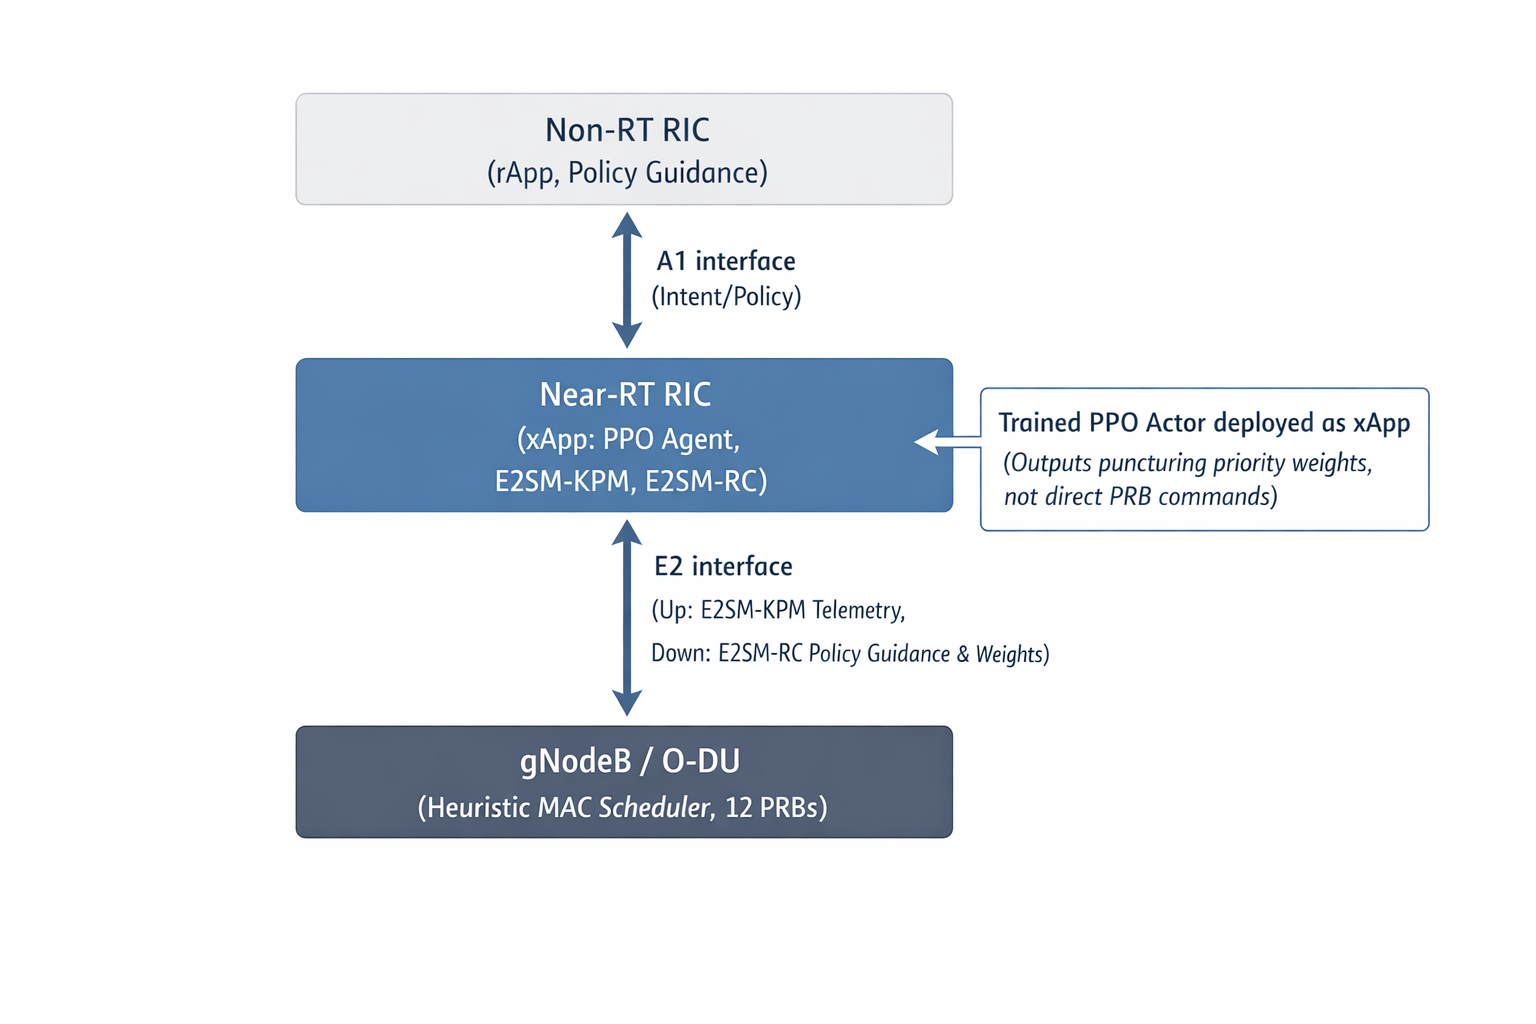
\includegraphics[width=0.9\textwidth]{O-RAN部署展望.png}
\caption{O-RAN 部署展望}
\label{fig:oran_deployment}
\end{figure}

基于本文的研究基础，后续工作可从算法优化与工程部署两个方向进一步拓展。

在算法层面，未来的改进可聚焦于提升模型的收敛性与泛化能力。一个直接方向是增加训练步数（Total Timesteps），以缓解当前 PPO 算法收敛不足的问题。作为同策略（on-policy）算法，PPO 依赖大量的交互样本来进行充分的策略探索与稳定的梯度估计，因此扩大采样规模是最直接的优化方向。另一个方向是引入课程学习（Curriculum Learning）机制来优化训练路径。结合本文在分布外鲁棒性测试中使用的离散到达率测试集 \(\Lambda_{\text{test}}=\{0.2,0.4,0.6,0.8,1.0,1.2,1.5\}\)，训练过程可以按照 URLLC 负载难度分阶段展开，也就是先让智能体在流量比较平稳的场景中学到基础的资源调度经验，形成一定的启发式先验（Heuristic Prior），再逐步过渡到高负载、长尾突发的非平稳（Non-stationary）流量环境中，让策略完成迁移；这样的训练顺序更平滑，能减少智能体在训练初期因为环境随机性过强而出现的大幅震荡。面对 5G/6G 中严格的 SLA 要求，后续还可以加入多目标约束强化学习，或者风险规避（Risk-Averse）强化学习（风险规避 RL）框架，把时延违约和可靠性下降带来的风险一起纳入算法底层控制中，从而提升智能体对服务质量风险的综合把握能力；最新综述研究也指出，面向 B5G 网络切片的多智能体深度强化学习（MADRL）在多域资源协同和自适应资源编排中有较大的应用潜力\cite{cui2026}。因此，本文提出的频域打孔负载均衡 PPO 思路，后续可以继续扩展到多智能体架构中，并结合联邦学习等分布式训练机制，在 O-RAN 云原生环境下进一步探索计算、通信和切片资源的联合闭环优化。

在工程应用层面，本文当前的 DRL 抢占策略已经在自建的 Gymnasium 仿真环境中得到验证，不过要把它进一步转化为具备落地潜力的 5G/6G 系统级方案，还需要考虑它在真实开放网络架构（如 O-RAN）中的跨平台逻辑映射。后续研究可以尝试把本文训练得到的 PPO 模型，从离线仿真环境迁移到近实时网络控制器中，并作为 AI 微服务（如 xApp）运行，具体的系统级映射关系可以从以下几个方面展开：

第一个方面是部署位置映射：模型从仿真交互环境向控制器微服务转化。 在本文实验中，智能体与环境进行理想化、同步的状态转移交互；真实系统部署时，底层的仿真环境会换成真实的基站物理节点，承载本文 Actor-Critic 神经网络权重的 PPO 智能体，可以作为独立推理模块放到网络控制器上，通过标准南向接口定期读取基站状态，再推理出面向 URLLC 和 eMBB 切片的宏观资源调配策略。

第二个方面是状态观测映射：从仿真中的理想可靠性裕度到延迟遥测数据。 在当前的 Gymnasium 环境中，状态空间包含 Perfect-CSI 假设下的 eMBB 码字理想可靠性裕度、剩余裕度、URLLC 实时队列和上一时步反馈等 rich observation；而在真实部署中，智能体需要通过订阅底层基站的周期性遥测数据来感知网络，CSI、CQI/MCS、BLER 预测、HARQ ACK/NACK 和译码反馈都可能带有估计误差和传输时延。也就是说，当模型拿到状态观测值时，真实物理信道和底层队列状态可能已经发生变化，所以后续算法需要明确处理估计误差、延迟观测，以及这些问题引出的部分可观测性风险。

第三个方面是动作输出的逻辑抽象：从离散抢占动作到策略指导（Policy Guidance）。 这是算法跨平台映射中比较关键、也比较难处理的一点；在本文的仿真环境中，PPO 智能体会在每一个微时隙（Mini-slot，亚毫秒级）做决策，并直接给出具体的离散频段（FR）抢占位置，这个动作落到物理层后就表现为对应的打孔效果。但在真实网络中，近实时控制器的控制环路通常超过 10 毫秒，明显慢于底层基站 MAC 调度器的微观调度频率，所以本文的 PPO 输出动作不能直接当成底层的``绝对 PRB 打孔执行指令''。

更合适的做法是先完成逻辑抽象，把 PPO 学到的``频域打孔负载均衡''经验，转换成底层 MAC 调度器可以使用的``策略指导''；例如，控制器上的智能体可以根据当前信道和 eMBB 码字的整体状态，向基站下发某个控制周期内的``打孔优先级权重''，或者给出``eMBB 容错安全余量建议''。当不可预测的 URLLC 突发包真正到达后，底层启发式 MAC 调度器就可以按照智能体下发的宏观策略，在毫秒级闭环内独立完成具体的物理层离散打孔操作；另一方面，随着基带处理单元（Baseband Unit, BBU）中的 AI 硬件加速能力逐渐成熟，比如边缘 NPU/FPGA 能力提升，后续研究也可以尝试把轻量级 DRL 推理模块作为内联服务（Inline Service），或者作为 O-DU 侧 dApp 下沉到 O-RAN 分布式单元（O-DU）中，这样就能在不跨越前传接口（Fronthaul）的情况下，实现真正的亚毫秒级（Sub-ms）微时隙闭环控制。

这种跨平台映射可以理解为：上层智能体先给出策略意图，底层调度器再执行更细的微观决策；这样一来，本文算法里把打孔压力分散到不同频域资源上的经验，就能进一步整理成更符合真实网络控制器时延限制的策略指导，也能为后面继续探索``算法离线训练---接口策略封装---硬件在环（Hardware-in-the-Loop）在线测试''的智能切片管理系统，提供一条比较清楚的实现路线。

\section{本章小结}\label{54-ux672cux7ae0ux5c0fux7ed3}

本章对全文研究内容作了整体梳理，围绕 eMBB/URLLC 联合切片场景中的 tolerance-aware MDP 建模、带有频域打孔负载均衡机制的奖励函数设计，以及基于 PPO 的抢占调度策略这三个方面，对本文研究问题给出了回应；同时结合基线对比和泛化测试结果，说明了本文算法在当前仿真条件下能达到的效果，以及它可能受到的性能边界。

一方面，本文也对当前研究中还不够充分的地方作了说明，包括模型训练步数有限、收敛还需要进一步加强，奖励函数权重仍带有人工设定的经验偏好，单小区抽象环境和 \(C_w\) 完美 CSI 上界假设仍偏理想化，以及在分布外（Out-of-Distribution, OOD）极端高负载突发流量下，模型的泛化能力还需要更多测试来验证；基于这些问题，后续可以从课程学习、多目标优化等方向继续改进算法。

在工程应用展望部分，本文还讨论了怎样把基于 Gymnasium 离线训练得到的 DRL 调度器，继续迁移到 O-RAN 开放架构中；这一部分重点说明模型作为微服务（xApp）运行在 Near-RT RIC 上时，可以采用什么样的部署思路，也梳理了从底层 E2SM-KPM 遥测状态订阅，到 E2SM-RC 策略指导下发的基本落地路径，同时指出可靠性裕度估计误差和反馈时延都会给真实部署带来挑战。

从整体上看，本文依托自建并扩展后的代码库，为 5G/6G 开放无线接入网中的切片资源分配，搭建了一个可以复现的深度强化学习仿真框架；这个框架在当前抽象 SLA 约束下，验证了数据驱动算法用于调度的潜力，也能给后续开发面向实际基站近实时智能控制的 QoS xApp，提供仿真层面的参考。










\printbibliography

\end{document}
